\documentclass[11pt]{article}

% --- packages ---
\usepackage[margin=1in]{geometry}
\usepackage{amsmath,amssymb,amsfonts}
\usepackage{booktabs}
\usepackage{graphicx}
\usepackage{hyperref}
\usepackage{xcolor}
\usepackage{multirow}
\usepackage{float}
\usepackage[numbers]{natbib}
\usepackage{algorithm}
\usepackage{algorithmic}
% \usepackage{microtype}  % disabled: MiKTeX font expansion issue
\usepackage{bookmark}

\hypersetup{
  colorlinks=true,
  linkcolor=blue!60!black,
  citecolor=blue!60!black,
  urlcolor=blue!60!black
}

% --- metadata ---
\title{%
  The Learnable Bridge:\\
  Cybernetic Feedback Discovers Rhombic Dodecahedral\\
  Geometry in Multi-Channel LoRA%
}

\author{%
  Timothy Paul Bielec%
  \thanks{Corresponding author. \texttt{timothy@promptcrafted.com}}%
  \\
  Promptcrafted LLC\\
  Los Angeles, CA
}

\date{March 2026}

\begin{document}
\maketitle

% ===================================================================
\begin{abstract}
Multi-channel LoRA (RhombiLoRA) partitions a low-rank adapter's
bottleneck into $n$ parallel channels and couples them through a
learnable $n \times n$ bridge matrix. We introduce the Steersman, a
cybernetic feedback mechanism that monitors the bridge's spectral
properties during training and encodes a geometric prior based on the
rhombic dodecahedron's 3-axis coordinate system. Across 13 experiments
spanning 1.1B--14B parameters, 60{,}000+ bridge matrices, and four
model scales (Qwen~1.5B, TinyLlama~1.1B, Qwen~7B, Wan~2.1~14B), the
Steersman at $n = 6$ produces 100\% block-diagonal bridge
structure---three independent $2 \times 2$ blocks aligned with the RD
coordinate axes---while non-cybernetic training produces 0\%.
Block-diagonal lock-in occurs within 200 training steps and is
independent of initialization strategy, including initializations that
actively oppose the target topology (I~Ching complementary trigrams
suppressed 99.5\% in 900 steps). Channel-count ablation across
$n \in \{3, 4, 6, 8\}$ reveals that the contrastive loss encoding RD
face-pair geometry is necessary and sufficient at $n = 6$: with
contrastive active, the co-planar/cross-planar coupling ratio reaches a
peak of 82{,}854:1 and Bridge Fiedler eigenvalue collapses to 0.00009;
at $n \in \{3, 4, 8\}$ (contrastive disabled), Bridge Fiedler converges
to ${\sim}0.09$ with 0\% block structure---a $1{,}020\times$
bifurcation. The discovered structure has effective dimensionality~3,
matching the number of coordinate axes: $n = 3$ achieves
matching validation loss to $n = 6$ (maximum delta: 0.16\% across 100
checkpoints) with $4\times$ fewer bridge parameters. Task performance is
orthogonal to bridge topology. The
Steersman reveals structural preferences that standard training does
not surface.
\end{abstract}

\noindent\textbf{Keywords:} low-rank adaptation, multi-channel LoRA,
cybernetic feedback, bridge matrix, block-diagonal structure,
rhombic dodecahedron, spectral graph theory, parameter-efficient fine-tuning

% ===================================================================
\section{Introduction}
\label{sec:intro}

Low-rank adaptation (LoRA)~\cite{hu2022lora} has become the dominant
method for parameter-efficient fine-tuning of large language models.
The standard formulation decomposes a weight update as
$\Delta W = BA$, where $B \in \mathbb{R}^{d \times r}$ and
$A \in \mathbb{R}^{r \times d}$ are low-rank projections and
$r \ll d$. This factorization is efficient, composable, and
well-understood. It is also structurally opaque: rank dimensions are
rotationally symmetric---for any orthogonal~$R$,
$BR^\top RA = BA$---and the adapter provides no compact representation
of the coupling structure it has learned.

Multi-channel extensions of LoRA partition the rank space into $n$
parallel channels of width $r/n$ and insert a learnable
$n \times n$ \textbf{bridge matrix} $\mathbf{M}$ between the down-
and up-projections. The bridge parameterizes inter-channel coupling:
$M_{ij}$ controls how strongly channel~$j$'s activations
influence channel~$i$'s output. When $\mathbf{M} = I_n$, channels
are independent and the architecture reduces to standard LoRA. When
$\mathbf{M}$ departs from the identity, the bridge encodes learned
relationships between channels---relationships that the training
objective and data jointly determine.

The bridge matrix creates a new object of study. Unlike the
high-dimensional projection matrices $A$ and $B$, the bridge is small
($n^2$ parameters per adapted module), invariant-rich (its
eigenspectrum is rotation-invariant), and directly interpretable (each
entry quantifies a specific inter-channel interaction). Preliminary
experiments established that untrained bridges learn task-discriminative
structure: a leave-one-out SVM on 28 query-projection bridges
(1{,}008 parameters) classifies task type at 84.5\% accuracy, and
bridge interpolation between adapters preserves eigenspectrum structure
(cosine similarity ${>}\,0.999$) at all mixing ratios
(Table~\ref{tab:experiments}, exp1a--e). Those preliminary experiments
also revealed a null result: without explicit supervision, the bridge
learns \emph{that} cross-channel coupling helps but not \emph{which}
channels to couple preferentially (co-planar/cross-planar
ratio $= 1.002$, $p = 0.474$).

This paper asks what happens when the bridge receives structured
feedback. We introduce the \textbf{Steersman}, a second-order
cybernetic feedback mechanism that monitors the bridge's spectral
properties during training and adjusts optimization dynamics
accordingly. The Steersman encodes a geometric prior derived from the
rhombic dodecahedron (RD): its 12 faces decompose into 3 pairs of
opposing faces along the $x$, $y$, and $z$ coordinate axes, and the
contrastive loss component rewards coupling between co-planar
face-pairs (channels sharing an axis) while penalizing coupling
between cross-planar pairs (channels on different axes). The spectral
component regularizes overall bridge connectivity via the Fiedler
eigenvalue. Together, these components define a target
topology---block-diagonal structure with three independent
$2 \times 2$ blocks---without directly imposing it.

The question is whether the bridge discovers this structure, and if
so, whether the discovery is consistent, fast, and mechanistically
attributable.

Across 6 cybernetic experiments encompassing 42{,}500+ bridge
matrices, 2 model scales (TinyLlama~1.1B, Qwen~7B), and 3
initialization strategies, the results are consistent:

\textbf{Block-diagonal emergence is robust.} Every cybernetic
experiment with $n = 6$ channels produces 100\% block-diagonal bridge
structure. Every non-cybernetic experiment (570~final-state bridges
across 3 model scales including Wan~2.1 at 14B) produces~0\%. The
Steersman is necessary and sufficient at $n = 6$.

\textbf{The structure is initialization-independent.} Three
initialization strategies---identity (no bias), geometric (weak
co-planar bias), and corpus-coupled (I~Ching complementary trigrams
that actively oppose the target topology)---converge to the same final
state: 100\% block-diagonal, co-planar/cross-planar ratios in the
64{,}000:1--71{,}000:1 band, and validation loss within 0.13\% of
each other. The corpus-coupled initialization starts with cross-planar
dominance; the Steersman inverts the coupling hierarchy within 75
steps and suppresses the opposing structure by 99.5\% within 900
steps (I~Ching complementary coupling:
$0.029 \to 0.0001$). Initialization effects vanish within 200~steps.

\textbf{Lock-in is fast.} Block-diagonal structure reaches 100\% by
step~200 in all experiments. Cross-planar coupling decays
exponentially with a half-life of 123~steps. Co-planar coupling grows
linearly. The topology is selected in the first 200 steps; the
remaining training deepens the separation, driving the
co-planar/cross-planar ratio from ${\sim}200$:1 at lock-in to a peak
of 82{,}854:1 (C-003, step~9{,}000) and a convergence band of
${\sim}70{,}000$:1 at 10{,}000~steps.

\textbf{Task performance is orthogonal to bridge topology.} Validation
loss at 10{,}000 steps is 0.4015--0.4022 across channel counts
$n \in \{3, 4, 6\}$, a maximum delta of 0.17\%. Block-diagonal
structure provides no measurable performance benefit. The bridge
topology is a structural signature, not a performance feature.

\textbf{The contrastive loss is necessary and sufficient at $n = 6$.}
Channel-count ablation ($n \in \{3, 4, 6, 8\}$) isolates the
mechanism. The contrastive loss component encodes RD face-pair
geometry and is defined only for $n = 6$; for $n \neq 6$ it returns
zero, leaving the Steersman with spectral regularization alone. The
result: $n = 6$ produces Bridge Fiedler eigenvalue~$0.00009$ with
70{,}404:1 co-planar/cross-planar ratio; $n \in \{3, 4, 8\}$
(spectral-only) produce Bridge Fiedler~${\sim}0.09$ with
${\sim}1$:1 ratio and 0\% block structure---a $1{,}020\times$
bifurcation in spectral connectivity.

\textbf{The effective dimensionality is~3.} At $n = 3$, the bridge
has 9~parameters (3 off-diagonal pairs). At $n = 6$ with contrastive
loss active, the Steersman drives 12 of 15 off-diagonal entries to
zero, leaving effectively 3 active degrees of freedom---the same count as
$n = 3$. Both channel counts produce matching validation loss
(maximum delta: 0.16\% across 100 checkpoints), but $n = 3$ uses
$4\times$ fewer bridge parameters (792 vs.\ 3{,}168 total across all
modules).

\textbf{The finding is scale-consistent.} Block-diagonal structure
appears at both 1.1B (TinyLlama) and 7B (Qwen) under cybernetic
training. The Holly Battery experiment (Wan~2.1, 14B~parameters,
video diffusion) without Steersman produces 0\% block structure at
co-planar/cross-planar ratio~1.07:1, providing additional evidence that the effect requires the
Steersman, not model scale or architecture alone.
Cross-layer correlation Fiedler converges to~${\sim}0.10$ for
cybernetic text models (0.102 at Qwen~7B, 0.101 at
TinyLlama)---a scale-consistent structural metric.

We make the following contributions:

\begin{enumerate}
  \item \textbf{Block-diagonal emergence as a consistent property of
    cybernetic multi-channel LoRA training.} 100\% block-diagonal
    structure across 6~experiments, 42{,}500+ bridges, 2~model scales,
    with 0\% in all non-cybernetic controls.
  \item \textbf{Initialization independence.} Three qualitatively
    different initialization strategies converge to the same
    block-diagonal attractor within 200~steps.
  \item \textbf{Coupling dynamics characterization.} Cross-planar
    coupling decays exponentially (half-life: 123~steps). Co-planar
    coupling grows linearly (${\sim}0.00012$/step). Peak ratio:
    82{,}854:1 (converged: ${\sim}70{,}000$:1).
  \item \textbf{Channel count as effective rank.} $n = 3$ matches
    $n = 6$ validation loss with $4\times$ fewer bridge parameters.
    Effective dimensionality equals the number of coordinate axes.
  \item \textbf{Contrastive loss as the mechanism (necessary and
    sufficient at $n = 6$).} Spectral regularization alone produces uniform coupling
    (Fiedler~${\sim}0.09$). Adding the contrastive component produces
    $1{,}020\times$ lower Fiedler ($0.00009$) and 70{,}000:1
    co-planar/cross-planar separation.
  \item \textbf{Scale consistency from 1.1B to 7B parameters.}
    Block-diagonal structure emerges consistently at TinyLlama~1.1B and
    Qwen~7B. Cross-layer Fiedler~${\sim}0.10$ at both cybernetic scales.
\end{enumerate}

The remainder of this paper is organized as follows.
Section~\ref{sec:background} reviews background and related work.
Section~\ref{sec:method} describes the RhombiLoRA architecture, the
Steersman feedback mechanism, and the RD geometry.
Section~\ref{sec:emergence} presents the core experimental evidence
for block-diagonal emergence.
Section~\ref{sec:ablation} reports the channel-count ablation.
Section~\ref{sec:scale} examines scale invariance.
Section~\ref{sec:discussion} discusses implications, limitations, and
connections to broader questions.
Section~\ref{sec:conclusion} concludes.


% ===================================================================
\section{Background and Related Work}
\label{sec:background}

\subsection{Low-Rank Adaptation}

LoRA~\cite{hu2022lora} injects trainable low-rank decompositions into
frozen pretrained models, reducing the number of trainable parameters
by orders of magnitude while maintaining competitive task performance.
The method has been extended along several axes: adaptive rank
allocation (AdaLoRA)~\cite{zhang2023adalora}, weight decomposition
(DoRA)~\cite{liu2024dora}, and multi-task composition
(LoRAHub)~\cite{huang2023lorahub}. All standard LoRA variants treat
the rank dimensions as a homogeneous vector space---individual rank
dimensions are interchangeable under rotation, and the adapter
provides no compact representation of inter-dimensional coupling.

\subsection{Multi-Channel and Multi-Head Parameter-Efficient Methods}

\begin{sloppypar}
Several works partition the adapter's parameter space into parallel
components. Multi-head LoRA~\cite{wang2024multihead} splits the rank
into heads that attend to different input subspaces.
Mixture-of-LoRA~\cite{li2024moe} routes inputs through multiple LoRA
experts.  These methods introduce structural decomposition but do not
include learnable inter-component coupling---each head or expert
operates independently, and the outputs are combined through fixed
aggregation (concatenation, addition, or gating).
MELoRA~\cite{ren2024melora} partitions the rank into mini-ensemble
channels that operate independently ($\mathbf{M} = I_n$); this is a
special case of the bridge formulation introduced below.
\end{sloppypar}

The closest architectural precedent is
LoRA-XS~\cite{banaei2024loraxs}, which places an $r \times r$ matrix
between $A$ and $B$ but freezes the outer projections to minimize
parameter count. Because $A$ and $B$ do not adapt to the task in
LoRA-XS, the intermediate matrix cannot serve as a diagnostic of what
joint $A$-$B$ learning discovered---it \emph{is} the entirety of
learned adaptation. RhombiLoRA trains all three components jointly
($A$, $B$, and an $n \times n$ bridge with $n \ll r$), enabling the
bridge to capture the emergent coupling pattern rather than carrying
the full adaptation burden.

RhombiLoRA introduces the bridge matrix as an explicit
parameterization of inter-channel coupling. Preliminary experiments
(Table~\ref{tab:experiments}, exp1a--e) established that the bridge
learns task-discriminative structure under standard (non-cybernetic)
training: bridge fingerprints classify task type with 84.5\%
leave-one-out accuracy, and bridge interpolation preserves
eigenspectrum structure at all mixing ratios. However, without
structured feedback, the bridge develops uniform coupling with no
topological preference (co-planar/cross-planar ratio~1.002:1). The
present work introduces the Steersman to provide that structured
feedback.

\subsection{Cybernetic Optimization}

Cybernetic control theory~\cite{wiener1948, ashby1956, beer1972}
formalizes feedback systems that maintain stability through
sense-decide-actuate loops. In machine learning, second-order feedback has appeared in
learning rate scheduling~\cite{smith2017cyclical}, loss landscape
analysis~\cite{li2018visualizing}, and
meta-learning~\cite{andrychowicz2016}. The Steersman differs from
learned meta-optimizers in that its control laws are fixed (not
learned), its state space is low-dimensional (3~scalar diagnostics),
and its actuation is limited to weight adjustments and learning rate
scaling. This simplicity is deliberate: we aim to demonstrate that
even minimal feedback is sufficient to drive strong structural
emergence.

\subsection{Block-Diagonal Structure in Neural Networks}

Block-diagonal weight matrices arise naturally in modular
networks~\cite{clune2013, amer2019modular}, where architectural
constraints enforce modularity. The lottery ticket
hypothesis~\cite{frankle2019lottery} identifies sparse subnetworks
within dense networks; when the surviving connections cluster, the
effective weight matrix is approximately block-diagonal. Mixture-of-experts
architectures~\cite{fedus2022switch, lepikhin2021gshard} achieve
block-diagonal routing through learned gating functions. In all these
cases, the block structure is either architecturally imposed (modular
networks), a consequence of pruning (lottery tickets), or mediated by
a separate routing mechanism (MoE gating). The present work
demonstrates block-diagonal emergence in a dense, unconstrained matrix
through feedback-driven training dynamics alone.

\subsection{The Rhombic Dodecahedron}

The rhombic dodecahedron (RD) is the Voronoi cell of the
face-centered cubic (FCC) lattice~\cite{conway1999}. Its 12 faces
tessellate $\mathbb{R}^3$ without gaps, and its dual is the
cuboctahedron. The RD's 6 face pairs partition naturally by coordinate
axis, yielding the 3-fold symmetry that motivates the contrastive loss
in Section~\ref{sec:steersman}. In prior
work~\cite{bielec2026shape}, we established that 12-connected FCC
lattices provide 30\% shorter paths and $2.4\times$ higher algebraic
connectivity than 6-connected cubic lattices at comparable spatial
resolution. A companion paper~\cite{bielec2026weights} showed that
structured edge weights aligned with the RD's 6 face-pair directions
amplify this advantage to $6.1\times$---the same directional structure
that motivates the contrastive loss in
Section~\ref{sec:steersman}. The present work uses the RD's coordinate
geometry as a structural prior for multi-channel coupling, not as a
spatial lattice.


% ===================================================================
\section{Method}
\label{sec:method}

\subsection{RhombiLoRA Architecture}

Standard LoRA~\cite{hu2022lora} decomposes each weight update as
$\Delta W = BA$, where $A \in \mathbb{R}^{r \times d_{\text{in}}}$
and $B \in \mathbb{R}^{d_{\text{out}} \times r}$ are low-rank factors
with rank~$r$. RhombiLoRA introduces a single additional component: a
learnable \emph{bridge matrix}
$\mathbf{M} \in \mathbb{R}^{n \times n}$ that couples $n$ parallel
channels within the low-rank bottleneck.

Given $n$ channels, the rank~$r$ is partitioned into $n$ equal
segments of size $s = r/n$ (we require $n \mid r$). The hidden
representation $\mathbf{h} = A\mathbf{x} \in \mathbb{R}^r$ is
reshaped into a matrix $\mathbf{H} \in \mathbb{R}^{n \times s}$,
where each row corresponds to one channel. The bridge acts on the
channel dimension:
%
\begin{equation}
  \mathbf{H}' = \mathbf{M} \mathbf{H}
\end{equation}

The coupled representation $\mathbf{H}'$ is flattened back to
$\mathbb{R}^r$ and projected through $B$. The complete forward pass
for a single RhombiLoRA adapter is:
%
\begin{equation}
  \Delta \mathbf{y} = \frac{\alpha}{r}\, B \cdot
    \mathrm{flatten}\!\bigl(\mathbf{M} \cdot
    \mathrm{reshape}(A\mathbf{x},\; [n, s])\bigr)
\end{equation}
%
where $\alpha$ is the LoRA scaling factor (set to~16 throughout). When
$\mathbf{M} = I_n$, channels are uncoupled and the forward pass
reduces exactly to standard LoRA. The bridge is initialized to
identity in all experiments unless otherwise noted.

Each attention projection within each transformer layer receives its
own independent bridge matrix. For a model with $L$ transformer layers
and four target projections per layer ($W_Q$, $W_K$, $W_V$, $W_O$),
the total number of bridge parameters is $n^2 \times 4 \times L$.
With $n = 6$, this yields $36 \times 4 \times 22 = 3{,}168$ bridge
parameters for TinyLlama-1.1B (22~layers) and
$36 \times 4 \times 28 = 4{,}032$ for Qwen2.5-7B-Instruct
(28~layers). These bridge parameters represent approximately 0.04\%
of the LoRA parameter budget.

The bridge parameterization is deliberately simple: a dense
$n \times n$ matrix with no architectural constraints such as
symmetry, positive definiteness, or sparsity. Any structure that
emerges in the learned bridge is a consequence of the training
dynamics, not of the parameterization.

\subsection{The Steersman: Cybernetic Feedback}
\label{sec:steersman}

Training proceeds with three loss components. The primary objective is
the standard causal language modeling loss~$\mathcal{L}_{\text{LM}}$.
Two auxiliary losses act on the bridge matrices: a contrastive
loss~$\mathcal{L}_{\text{con}}$ that encodes geometric priors, and a
spectral loss~$\mathcal{L}_{\text{spec}}$ that regularizes algebraic
connectivity. The total loss is:
%
\begin{equation}
  \mathcal{L} = \mathcal{L}_{\text{LM}} +
    w_c\, \mathcal{L}_{\text{con}} +
    w_s\, \mathcal{L}_{\text{spec}}
\end{equation}
%
where the weights $w_c$ and $w_s$ are not fixed hyperparameters but
are adjusted dynamically by the Steersman.

\paragraph{Contrastive loss.}
For $n = 6$, the bridge's off-diagonal entries are partitioned into
\emph{co-planar pairs} and \emph{cross-planar pairs} according to the
rhombic dodecahedral geometry described in
Section~\ref{sec:rdgeometry}. The contrastive loss encourages
co-planar coupling to exceed cross-planar coupling:
%
\begin{equation}
  \mathcal{L}_{\text{con}} = -\frac{1}{|\mathcal{A}|}
    \sum_{a \in \mathcal{A}} \left(
      \frac{1}{|\mathcal{C}|}\sum_{(i,j) \in \mathcal{C}} |M^a_{ij}|
      - \frac{1}{|\mathcal{X}|}\sum_{(i,j) \in \mathcal{X}} |M^a_{ij}|
    \right)
\end{equation}
%
where $\mathcal{A}$ is the set of all adapters, $\mathcal{C}$ is the
set of 3~co-planar index pairs, and $\mathcal{X}$ is the set of
12~cross-planar index pairs. For $n \neq 6$, the contrastive loss is
undefined and returns zero.

\paragraph{Spectral loss.}
The spectral regularization drives the algebraic
connectivity~\cite{fiedler1973} of each bridge toward a target Fiedler
eigenvalue~$\lambda_2^*$. For each
adapter~$a$, we construct the weighted Laplacian~$\mathbf{L}^a$ by
treating $|M^a_{ij}|$ ($i \neq j$) as edge weights of a complete
graph on $n$~nodes. The Fiedler value~$\lambda_2^a$ is the
second-smallest eigenvalue of~$\mathbf{L}^a$, computed via
\texttt{torch.linalg.eigvalsh} to maintain differentiability:
%
\begin{equation}
  \mathcal{L}_{\text{spec}} = \frac{1}{|\mathcal{A}|}
    \sum_{a \in \mathcal{A}} (\lambda_2^a - \lambda_2^*)^2
\end{equation}
%
The initial target is $\lambda_2^* = 0.1$; this is adapted upward
during training to track the observed mean Fiedler value.

\paragraph{The Steersman.}
Every $T = 100$ training steps, the Steersman executes a
sense-decide-actuate cycle. During sensing, it extracts all bridge
matrices and computes: the mean Fiedler eigenvalue~$\bar{\lambda}_2$
across adapters, the mean co-planar to cross-planar coupling ratio,
and the mean Frobenius deviation from identity
$\|\mathbf{M} - I_n\|_F$. From a sliding window of the most recent
5~measurements, it estimates linear trends for each diagnostic.

Three control laws determine the actuator outputs:

\begin{enumerate}
  \item \emph{Connectivity.} If the Fiedler trend is declining
    (slope $< -0.001$), the spectral weight~$w_s$ is increased
    proportionally, bounded above by $w_s^{\max} = 0.2$. If the trend
    is positive, $w_s$ decays slowly toward its base value of~0.05.
  \item \emph{Directionality.} If the co-planar/cross-planar ratio is
    near unity and stagnating (trend magnitude ${<}\,0.02$), the
    contrastive weight~$w_c$ is increased, bounded above by
    $w_c^{\max} = 0.5$. Once the ratio exceeds~1.2, $w_c$ decays.
  \item \emph{Stability.} If the deviation from identity grows faster
    than a threshold (slope ${>}\,0.05$), the learning rate for bridge
    parameters is dampened multiplicatively (bounded below at
    $0.1\times$ the base rate).
\end{enumerate}

The Steersman's control laws are purely reactive: they adjust weights
and learning rates based on measured trends, with no model of the
system's future dynamics. The initial contrastive weight is
$w_c = 0.1$ and the initial spectral weight is $w_s = 0.05$.

\paragraph{Optimizer configuration.}
Bridge parameters and LoRA parameters ($A$, $B$) are placed in
separate optimizer parameter groups within a single AdamW optimizer
(weight decay~0.01). Both groups share a base learning rate of
$2 \times 10^{-4}$ with cosine decay after a linear warmup of
200~steps. The Steersman's bridge learning rate scaling (control
law~3) is applied as a multiplicative factor on the bridge parameter
group only.

\subsection{Rhombic Dodecahedral Geometry and Co-planar Pairs}
\label{sec:rdgeometry}

The rhombic dodecahedron is a convex polyhedron with 12 congruent
rhombic faces, 14~vertices (8~cubic and 6~octahedral), and 24~edges.
Its faces partition naturally into 6 antipodal pairs, each pair
sharing a common coordinate axis. In the standard embedding, the
6~face-pair normals align with the FCC lattice directions:
$(\pm 1, \pm 1, 0)$, $(\pm 1, 0, \pm 1)$, and
$(0, \pm 1, \pm 1)$. These 6~direction pairs are the channels of
RhombiLoRA when $n = 6$.

The 6 face pairs decompose further into 3 groups of 2 by the
coordinate that vanishes in their normal vectors:
%
\begin{itemize}
  \item $z{=}0$ group: channels $(0, 1)$, normals $(1,1,0)$ and $(1,-1,0)$
  \item $y{=}0$ group: channels $(2, 3)$, normals $(1,0,1)$ and $(1,0,-1)$
  \item $x{=}0$ group: channels $(4, 5)$, normals $(0,1,1)$ and $(0,1,-1)$
\end{itemize}
%
Two face pairs are \emph{co-planar} if they share a coordinate axis
(3~pairs). Two face pairs are \emph{cross-planar} if they lie on
different coordinate axes ($\binom{6}{2} - 3 = 12$ pairs). The
contrastive loss uses this partition directly.

The co-planar to cross-planar coupling ratio is defined as:
%
\begin{equation}
  \rho = \frac{
    \frac{1}{|\mathcal{C}|}\sum_{(i,j) \in \mathcal{C}} |M_{ij}|
  }{
    \frac{1}{|\mathcal{X}|}\sum_{(i,j) \in \mathcal{X}} |M_{ij}|
  }
  \label{eq:rho}
\end{equation}
%
where $\mathcal{C}$ denotes the 3~co-planar pairs and $\mathcal{X}$
denotes the 12~cross-planar pairs. A bridge with no directional
preference has $\rho \approx 1$. A perfectly block-diagonal bridge has
$\rho \to \infty$. We classify a bridge as block-diagonal if
$\rho > 10$ and every cross-planar entry has absolute value below
$10^{-3}$.

\subsection{Training Setup}
\label{sec:setup}

All experiments use the alpaca-cleaned dataset~\cite{alpaca} for
instruction-following fine-tuning. Models are loaded in bfloat16
precision with gradient checkpointing enabled. The base model
parameters are frozen; only the injected LoRA adapters (and their
bridge matrices) receive gradients.

Common hyperparameters: learning rate $2 \times 10^{-4}$, batch
size~2, gradient accumulation~8 (effective batch size~16), linear
warmup for 200~steps followed by cosine decay, maximum gradient
norm~1.0, LoRA rank~24, LoRA~$\alpha$~16, target modules
$\{W_Q, W_K, W_V, W_O\}$, random seed~42, maximum sequence
length~512.

The primary model is TinyLlama-1.1B-Chat (22~transformer layers,
88~adapters, 3{,}168~bridge parameters at $n = 6$). Scale validation
uses Qwen2.5-7B-Instruct (28~layers, 112~adapters, 4{,}032~bridge
parameters). A non-cybernetic control at 14B~scale uses Wan~2.1
(video diffusion backbone, 40~layers, no Steersman).

Three initialization strategies are tested:
\emph{Identity}~($\mathbf{M} = I_n$, equivalent to standard LoRA at
start).
\emph{Geometric}~($\mathbf{M} = I_6 + 0.01 \cdot \hat{C}$, weak
co-planar bias).
\emph{Corpus-coupled}~(off-diagonal entries from I~Ching
complementary trigram pairings, actively opposing the target topology
with I~Ching/RD ratio~1.4:1 at initialization).

The channel count ablation varies $n \in \{3, 4, 6, 8\}$ while
holding the total rank fixed at~24 (channel sizes
$s \in \{8, 6, 4, 3\}$). Because the contrastive loss is defined only
for $n = 6$, experiments with $n \neq 6$ operate under spectral
regularization alone---a deliberate experimental design that isolates
the geometric prior from the spectral pressure.


% ===================================================================
\section{Block-Diagonal Emergence}
\label{sec:emergence}

\subsection{Core Finding: Cybernetic vs.\ Non-Cybernetic Training}

With these components in place---multi-channel bridge, contrastive and
spectral losses, reactive feedback---we turn to the experimental
evidence.

Table~\ref{tab:experiments} presents the complete experimental record.
Across 13~experiments spanning four model scales, two training
regimes, four channel counts, and three initialization strategies, the
block-diagonal classification is binary: every cybernetic experiment
at $n = 6$ produces 100\% block-diagonal bridge structure, and every
other configuration produces~0\%.

\begin{table}[H]
\centering
\caption{Complete experiment summary. $\rho$ = co-planar/cross-planar
  coupling ratio. BD\% = percentage of bridges classified as
  block-diagonal ($\rho > 10$ and all cross-planar entries
  ${<}\,10^{-3}$).}
\label{tab:experiments}
\small
\begin{tabular}{llclccccc}
\toprule
ID & Model & $n$ & Init & Steersman & Steps & Val Loss & $\rho$ & BD\% \\
\midrule
exp1a--e & Qwen 1.5B & 6 & various & No & 2K & --- & ${\sim}1$:1 & 0\% \\
exp2 & Qwen 7B & 6 & FCC & No & 10K & --- & ${\sim}1$:1 & 0\% \\
exp2.5 & Qwen 7B & 6 & geometric & No & 3K & --- & ${\sim}1$:1 & 0\% \\
\midrule
\textbf{exp3} & \textbf{Qwen 7B} & \textbf{6} & identity & \textbf{Yes} & \textbf{12.9K} & --- & \textbf{18{,}248:1} & \textbf{100\%} \\
\textbf{exp3\_tiny} & \textbf{TinyLlama} & \textbf{6} & identity & \textbf{Yes} & \textbf{10K} & --- & \textbf{37{,}929:1} & \textbf{100\%} \\
\textbf{C-001} & \textbf{TinyLlama} & \textbf{6} & identity & \textbf{Yes} & \textbf{4K} & 0.4178 & \textbf{10{,}118:1} & \textbf{100\%} \\
\textbf{C-002} & \textbf{TinyLlama} & \textbf{6} & geometric & \textbf{Yes} & \textbf{10K} & \textbf{0.4010} & \textbf{71{,}337:1} & \textbf{100\%} \\
\textbf{C-003} & \textbf{TinyLlama} & \textbf{6} & corpus & \textbf{Yes} & \textbf{10K} & \textbf{0.4011} & \textbf{64{,}168:1} & \textbf{100\%} \\
\textbf{H3} & \textbf{TinyLlama} & \textbf{6} & identity & \textbf{Yes} & \textbf{10K} & \textbf{0.4015} & \textbf{70{,}404:1} & \textbf{100\%} \\
\midrule
H1 & TinyLlama & 3 & identity & Yes & 10K & 0.4020 & N/A & N/A \\
H2 & TinyLlama & 4 & identity & Yes & 10K & 0.4022 & ${\sim}1$:1 & 0\% \\
H4 & TinyLlama & 8 & identity & Yes & 10K & 0.4024 & ${\sim}1$:1 & 0\% \\
\midrule
Holly & Wan 2.1 14B & 6 & identity & No & 10 ep & 1.493 & 1.07:1 & 0\% \\
\bottomrule
\end{tabular}
\end{table}

Six cybernetic experiments at $n = 6$ contribute 42{,}500+ bridge
matrices. Each matrix is classified as block-diagonal if $\rho > 10$
(where $\rho$ is the co-planar to cross-planar coupling ratio, i.e.,
same-axis vs.\ different-axis channel pairs) and all cross-planar
entries fall below $10^{-3}$. The classification
rate is 100.0\% in every experiment, at every checkpoint from
step~200 onward. There are no exceptions, no near-misses, and no
late-onset failures. The attractor is robust across all tested
conditions.

Six non-cybernetic experiments contribute 570 final-state bridges.
None exhibits block-diagonal structure. Co-planar/cross-planar ratios
range from 0.99:1 to 1.07:1---statistically indistinguishable from
uniform coupling. The Holly Battery experiment (Wan~2.1~14B, Prodigy
optimizer, no Steersman) achieves 3.8\% lower loss than the non-RhombiLoRA baseline while using 9.15\,GB less VRAM and producing
6\% faster inference, but its bridge matrices remain near-identity
with $\rho = 1.07$:1. Performance benefits from multi-channel
parameterization do not require---and do not induce---topological
structure.

\subsection{Lock-in Dynamics}

Block-diagonal structure does not emerge gradually. It locks in within
200 training steps---2\% of total training---across all six cybernetic
$n = 6$ experiments.

Figure~\ref{fig:cybernetic} shows the co-planar/cross-planar ratio on
a logarithmic scale for all six experiments. Despite spanning two
model scales and three initialization strategies, the trajectories
are qualitatively identical: rapid exponential growth in the first
200~steps, followed by sustained linear growth on the log scale. By
step~200, every experiment exceeds $\rho = 100$:1. By step~1{,}000,
every experiment exceeds $\rho = 5{,}000$:1.

\begin{figure}[ht]
\centering
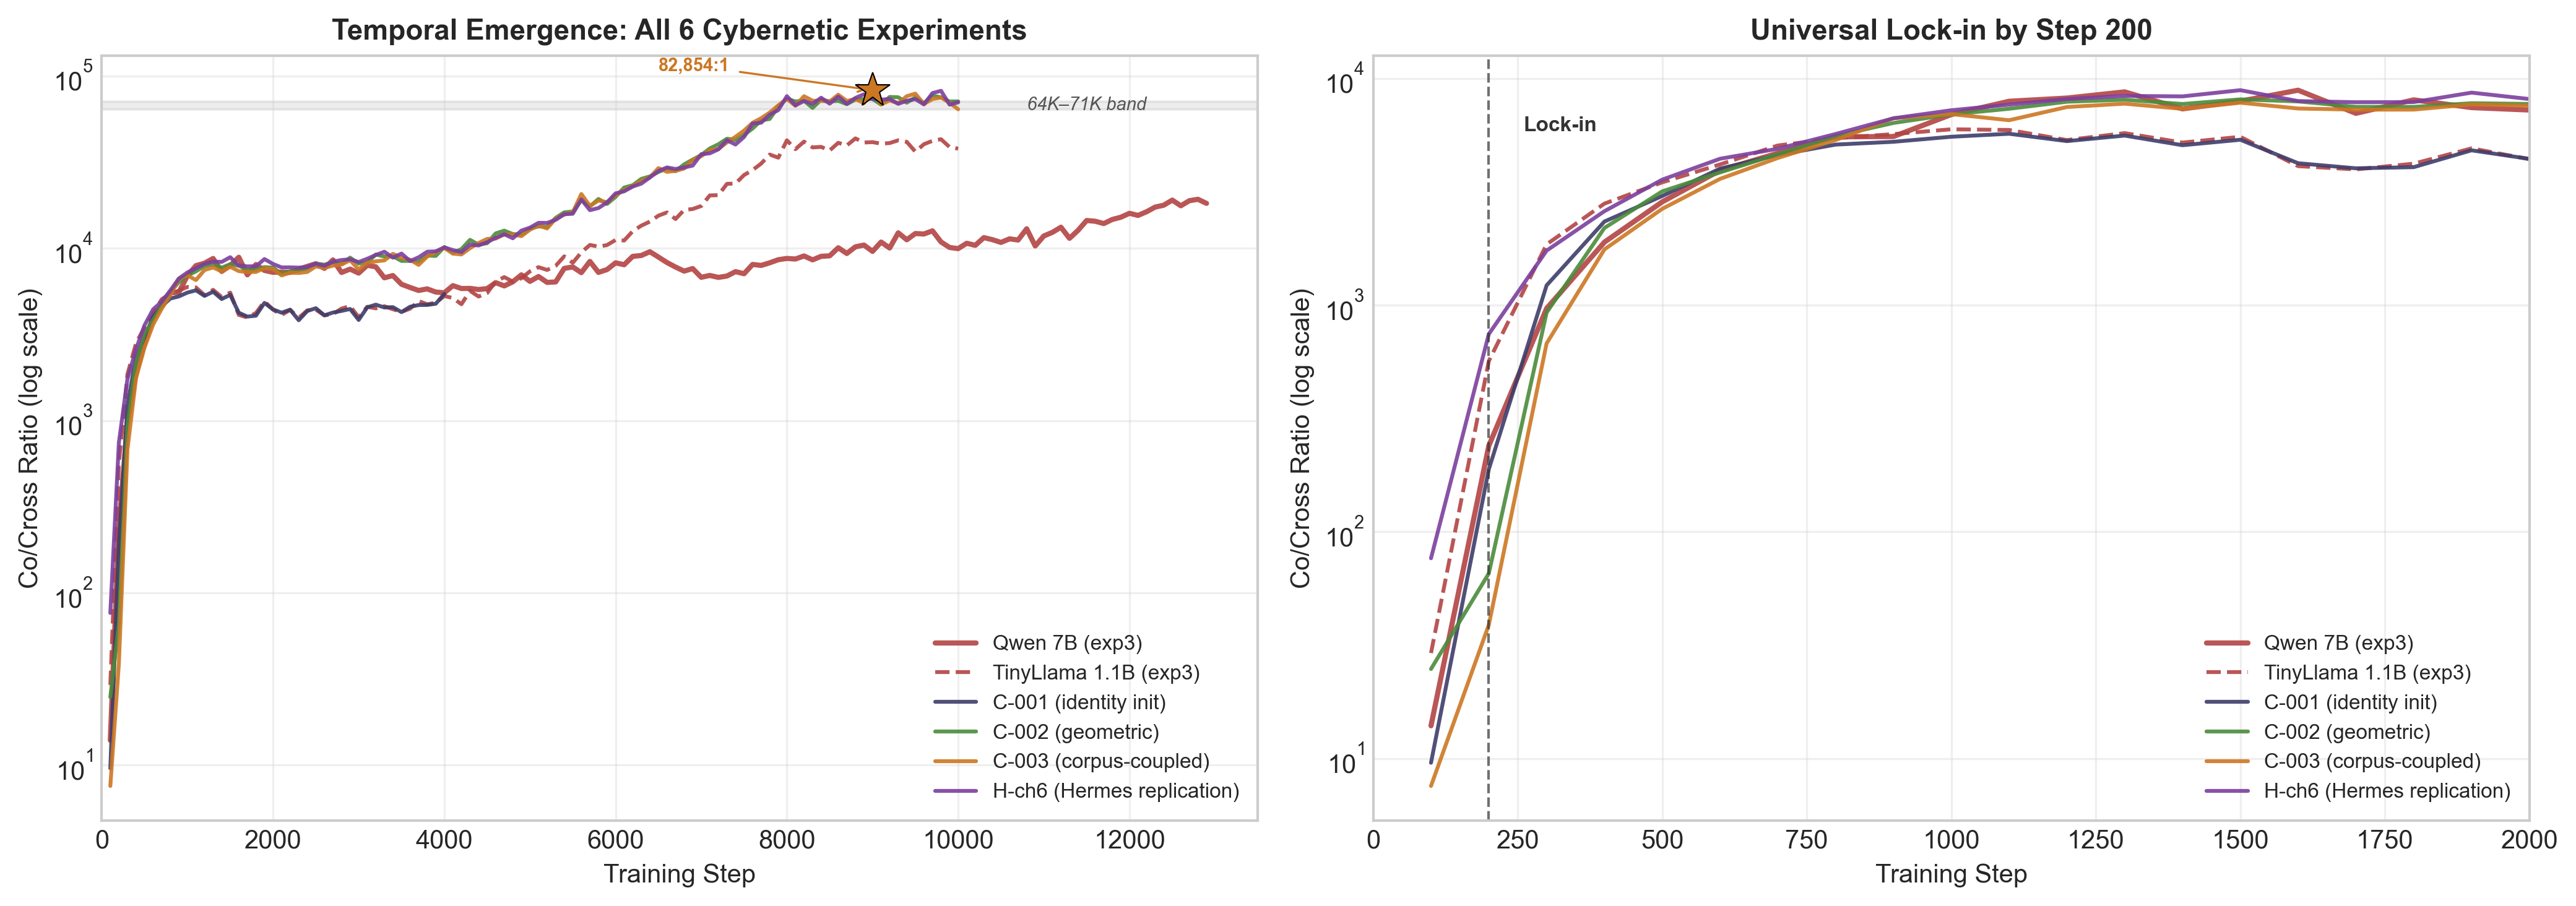
\includegraphics[width=0.85\textwidth]{figures3/fig1-cybernetic-overview}
\caption{Co-planar/cross-planar coupling ratio (log scale) for all
  six cybernetic $n = 6$ experiments. Lock-in occurs by step~200.
  Convergence band at 10{,}000~steps: 64{,}168:1--71{,}337:1. Peak:
  82{,}854:1 (C-003, step~9{,}000). The exp3 (Qwen~7B) lower ratio
  reflects an earlier code version, not a scale-dependent effect.}
\label{fig:cybernetic}
\end{figure}

The coupling dynamics decompose into two independent processes.
Cross-planar coupling decays exponentially from its initial value to a
computational floor of~${\sim}10^{-5}$. A least-squares fit across
three experiments (C-001, C-002, C-003) yields a consistent half-life
of $\tau_{1/2} = 123 \pm 8$~steps. Co-planar coupling grows linearly
at approximately $0.00012$ per step (Frobenius norm per module), with
no evidence of saturation through 10{,}000~steps ($R^2 = 0.998$ for
a linear fit from step~500 onward).

These two processes are independent: topology selection (which entries
are suppressed) occurs in the exponential phase and completes by
step~200; magnitude growth (how large the surviving entries become)
continues throughout training and drives the ratio upward. The peak
ratio is 82{,}854:1 (C-003, step~9{,}000). The peak does not occur
at the final step because cross-planar entries at the computational
floor exhibit stochastic fluctuations.

The final ratios at 10{,}000~steps for the three complete TinyLlama
runs converge to a narrow band: C-002~=~71{,}337:1,
H3~=~70{,}404:1, C-003~=~64{,}168:1 (maximum pairwise delta: 11\%).

\subsection{Initialization Independence}

The Steersman's block-diagonal attractor is strong enough to overwrite
any initial bridge structure. We test three strategies of increasing
adversarial strength.

\textbf{Identity initialization} ($\mathbf{M} = I_6$). Channels start
uncoupled. All off-diagonal entries begin at zero. The bridge must
discover both the topology and the dynamics from the training signal
and feedback alone.

\textbf{Geometric initialization}
($\mathbf{M} = I_6 + 0.01\, \hat{C}$). A small perturbation in the
direction of co-planar coupling. The perturbation magnitude~(0.01) is
two orders of magnitude below the final co-planar
coupling~(${\sim}1.4$ at step~10{,}000).

\textbf{Corpus-coupled initialization.} Off-diagonal entries are set
according to I~Ching complementary trigram pairings, producing a
bridge that initially favors cross-planar coupling (I~Ching/RD ratio
1.4:1 at step~0). This initialization \emph{opposes} the target
topology.

\begin{figure}[ht]
\centering
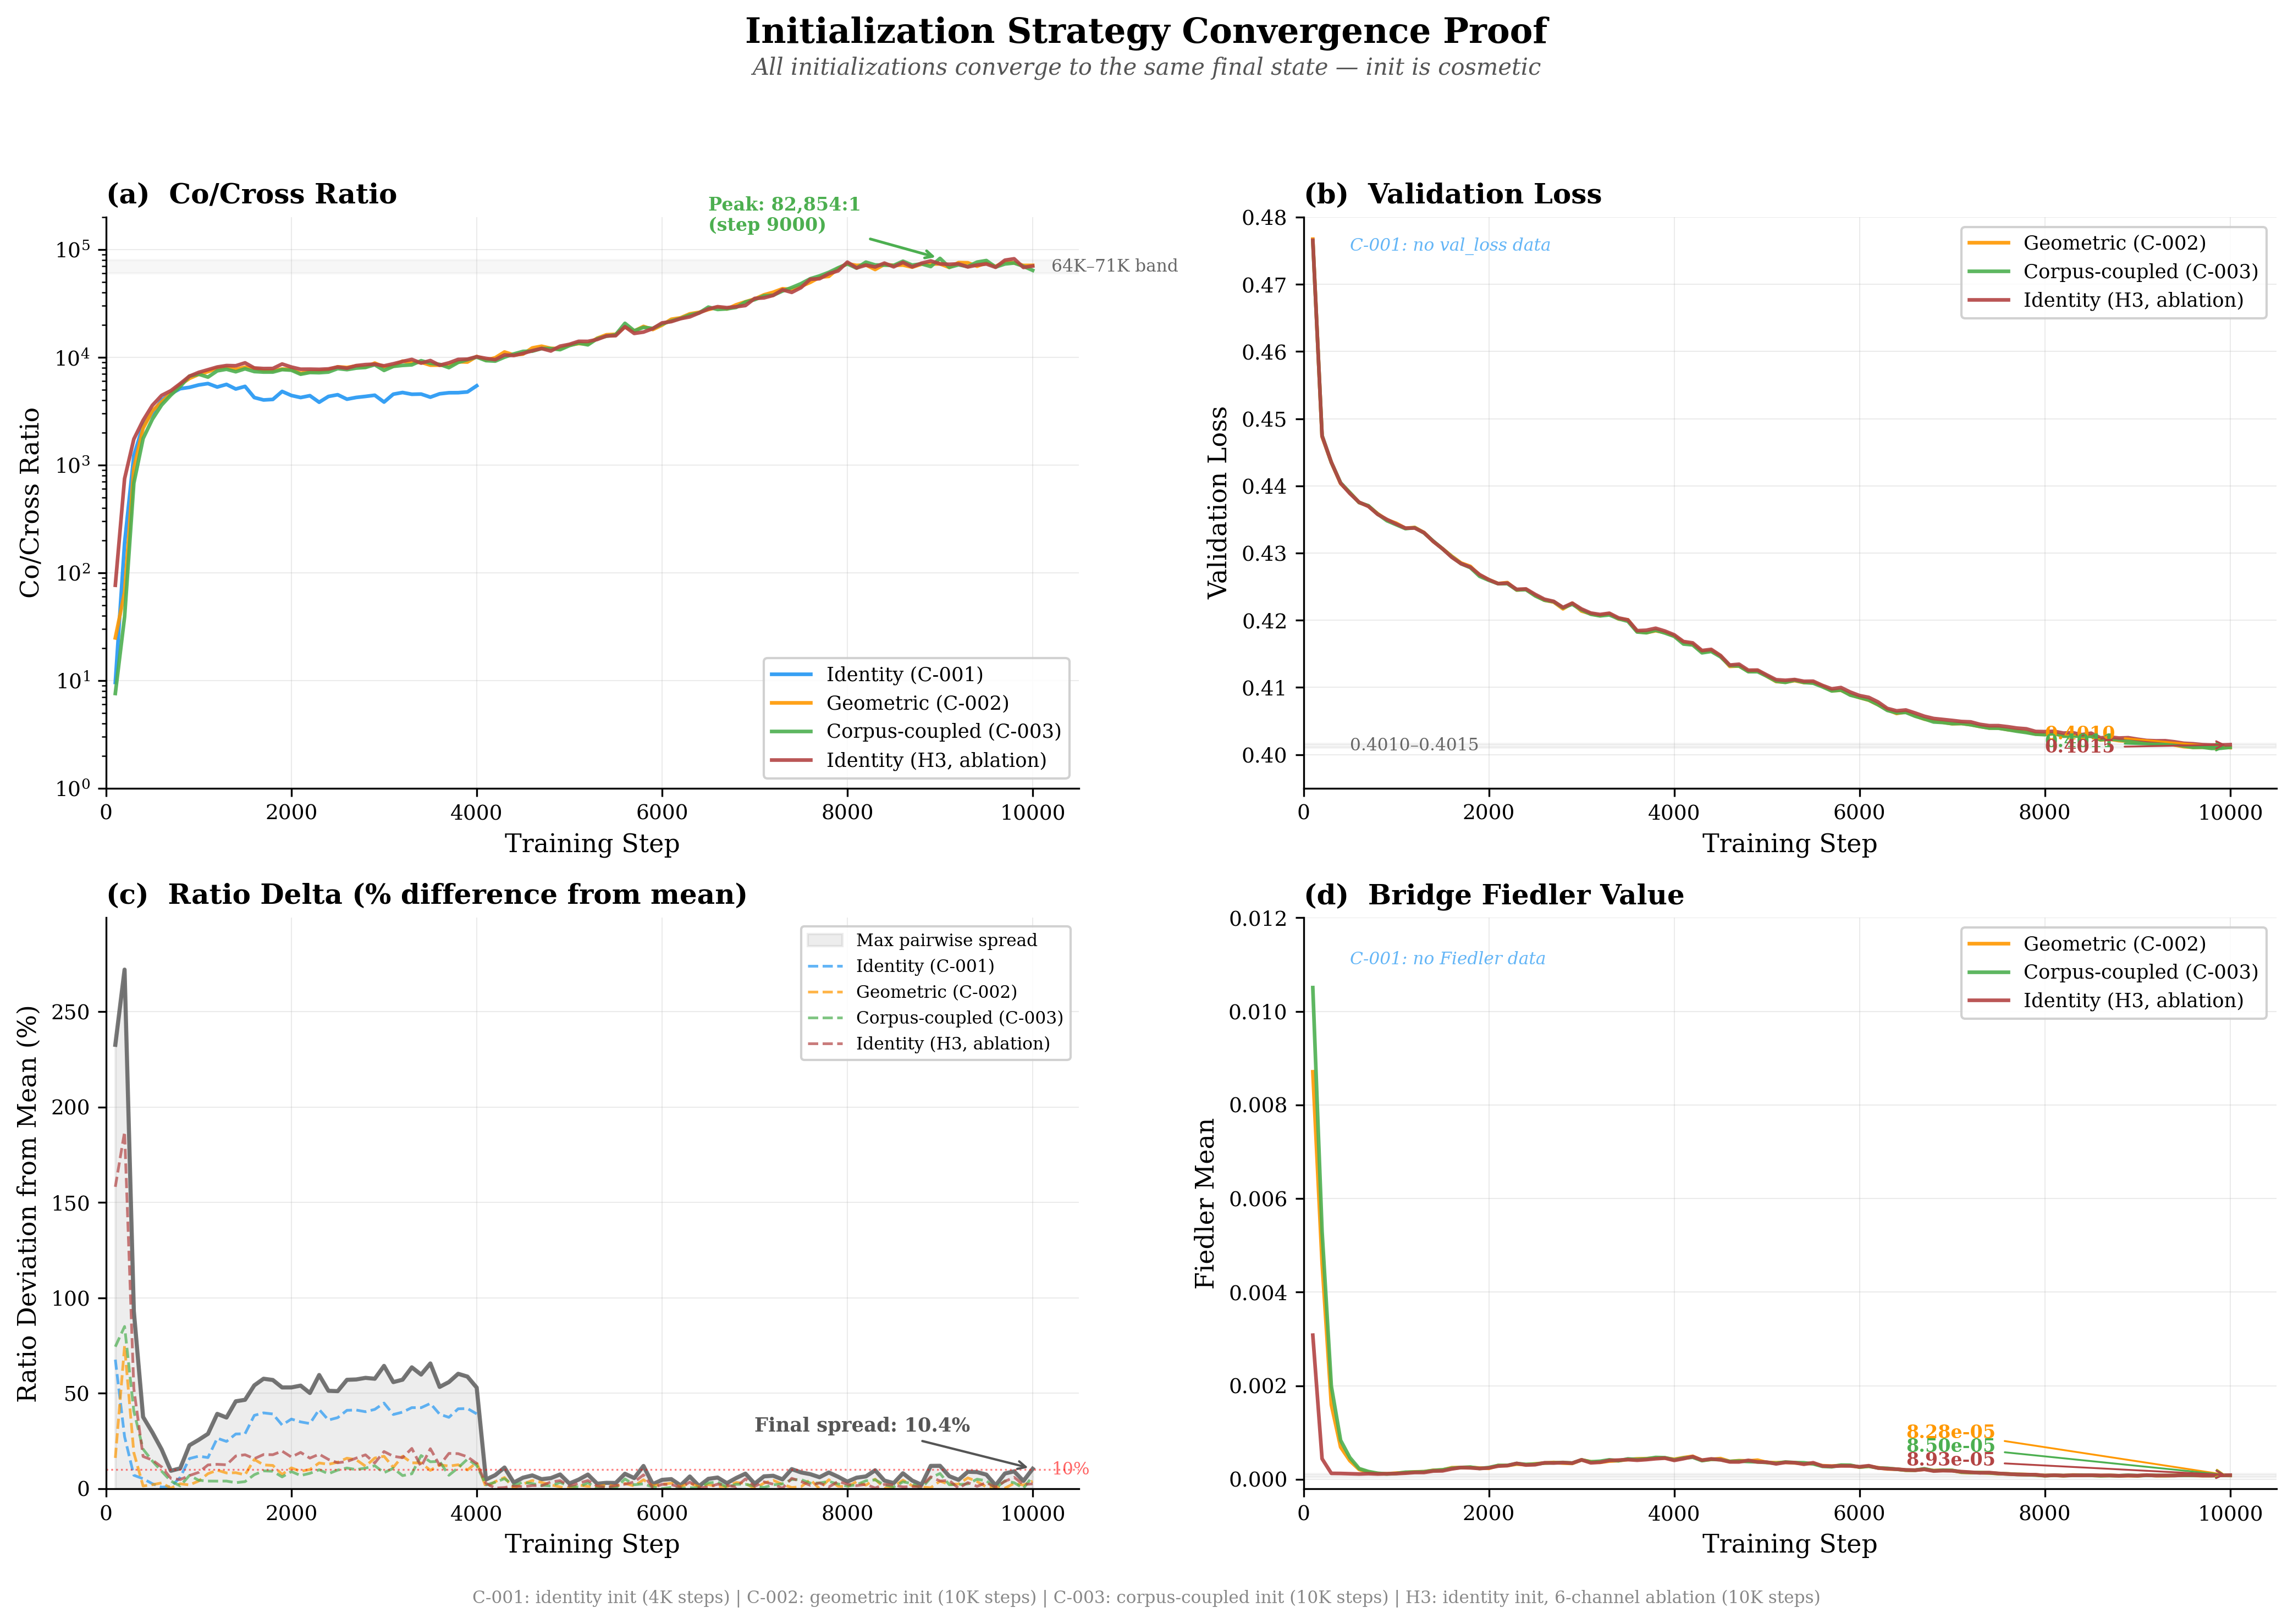
\includegraphics[width=0.85\textwidth]{figures3/fig2-init-convergence}
\caption{Four-panel initialization convergence evidence. All three
  strategies (C-001: identity, C-002: geometric, C-003: corpus)
  converge to the same attractor. Top-left: co-planar/cross-planar
  ratio. Top-right: validation loss. Bottom-left: ratio delta
  (\%). Bottom-right: Bridge Fiedler eigenvalue.}
\label{fig:init}
\end{figure}

All three initializations converge to the same final state
(Figure~\ref{fig:init}). At step~2{,}000, co-planar coupling
magnitudes for C-001, C-002, and C-003 are 0.252, 0.256, and 0.252
(maximum pairwise delta: 1.6\%). Final validation losses are
0.4178 (C-001, 4K~steps), 0.4010 (C-002, 10K), and 0.4011 (C-003,
10K). The convergence of C-002 and C-003 is within 0.025\% in
validation loss and 11\% in ratio.

The corpus-coupled experiment (C-003) provides the most detailed view
of attractor dynamics. Figure~\ref{fig:dismantling} tracks the
per-pair coupling magnitudes. At step~0, I~Ching complementary pairs
have combined coupling~0.029 (three pairs), while RD co-planar pairs
have combined coupling~0.020---a 1.4:1 disadvantage, consistent with
the initialization specification. By step~75, the RD pairs overtake
the I~Ching pairs. By step~200, I~Ching coupling has been suppressed
to~0.006 (79\% reduction). By step~900, it reaches~0.0001---a 99.5\%
reduction. The Steersman exponentially suppresses the opposing
structure while linearly growing the target structure.

\begin{figure}[ht]
\centering
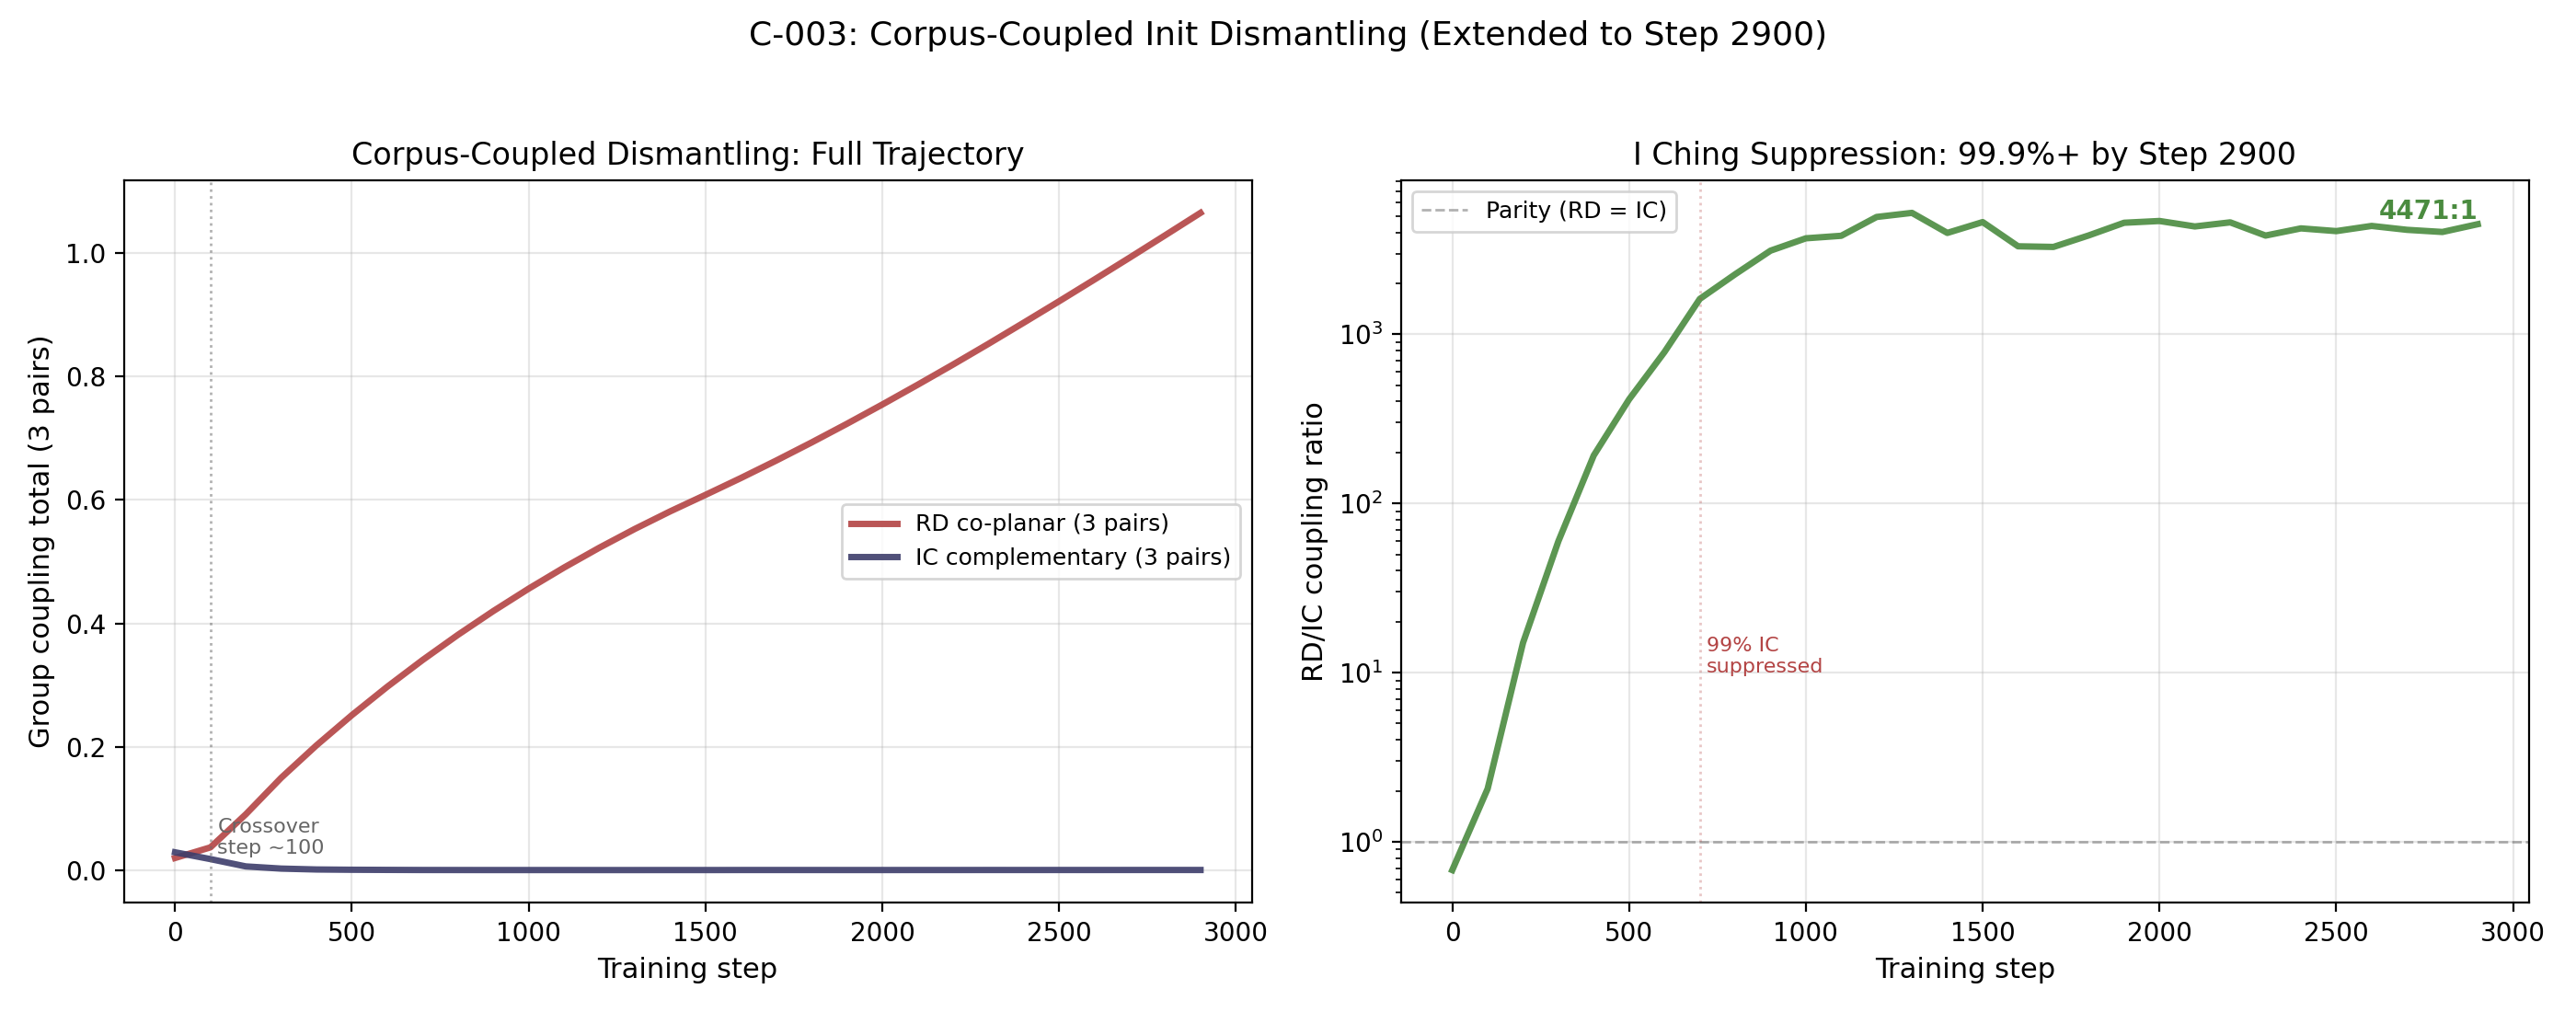
\includegraphics[width=0.75\textwidth]{figures3/fig3-corpus-dismantling}
\caption{Corpus-coupled dismantling (C-003). Per-pair coupling
  trajectories showing I~Ching$\to$RD crossover at step~${\sim}75$
  and 99.5\% suppression by step~900.}
\label{fig:dismantling}
\end{figure}

\subsection{Axis Symmetry and Polarity}

The block-diagonal structure exhibits two additional symmetries.
\textbf{Axis symmetry:} the three co-planar axes develop coupling of
equal magnitude (maximum deviation ${<}\,2.5\%$ across all
experiments and checkpoints). \textbf{Polarity freedom:} within each
$2 \times 2$ block, the off-diagonal entry can be positive or
negative (approximately 50/50 split). The Steersman constrains
\emph{which} channels couple but not \emph{how} they couple. This is
consistent with the contrastive loss operating on absolute values.

The combination of equal-magnitude axes with free polarity means the
Steersman discovers a 3-degree-of-freedom system embedded in a
15-degree-of-freedom parameter space. Each degree of freedom
corresponds to a coordinate axis.
Figure~\ref{fig:heatmaps} shows representative bridge matrices from
cybernetic and non-cybernetic training, illustrating the
$3 \times (2 \times 2)$ block-diagonal structure.

\begin{figure}[ht]
\centering
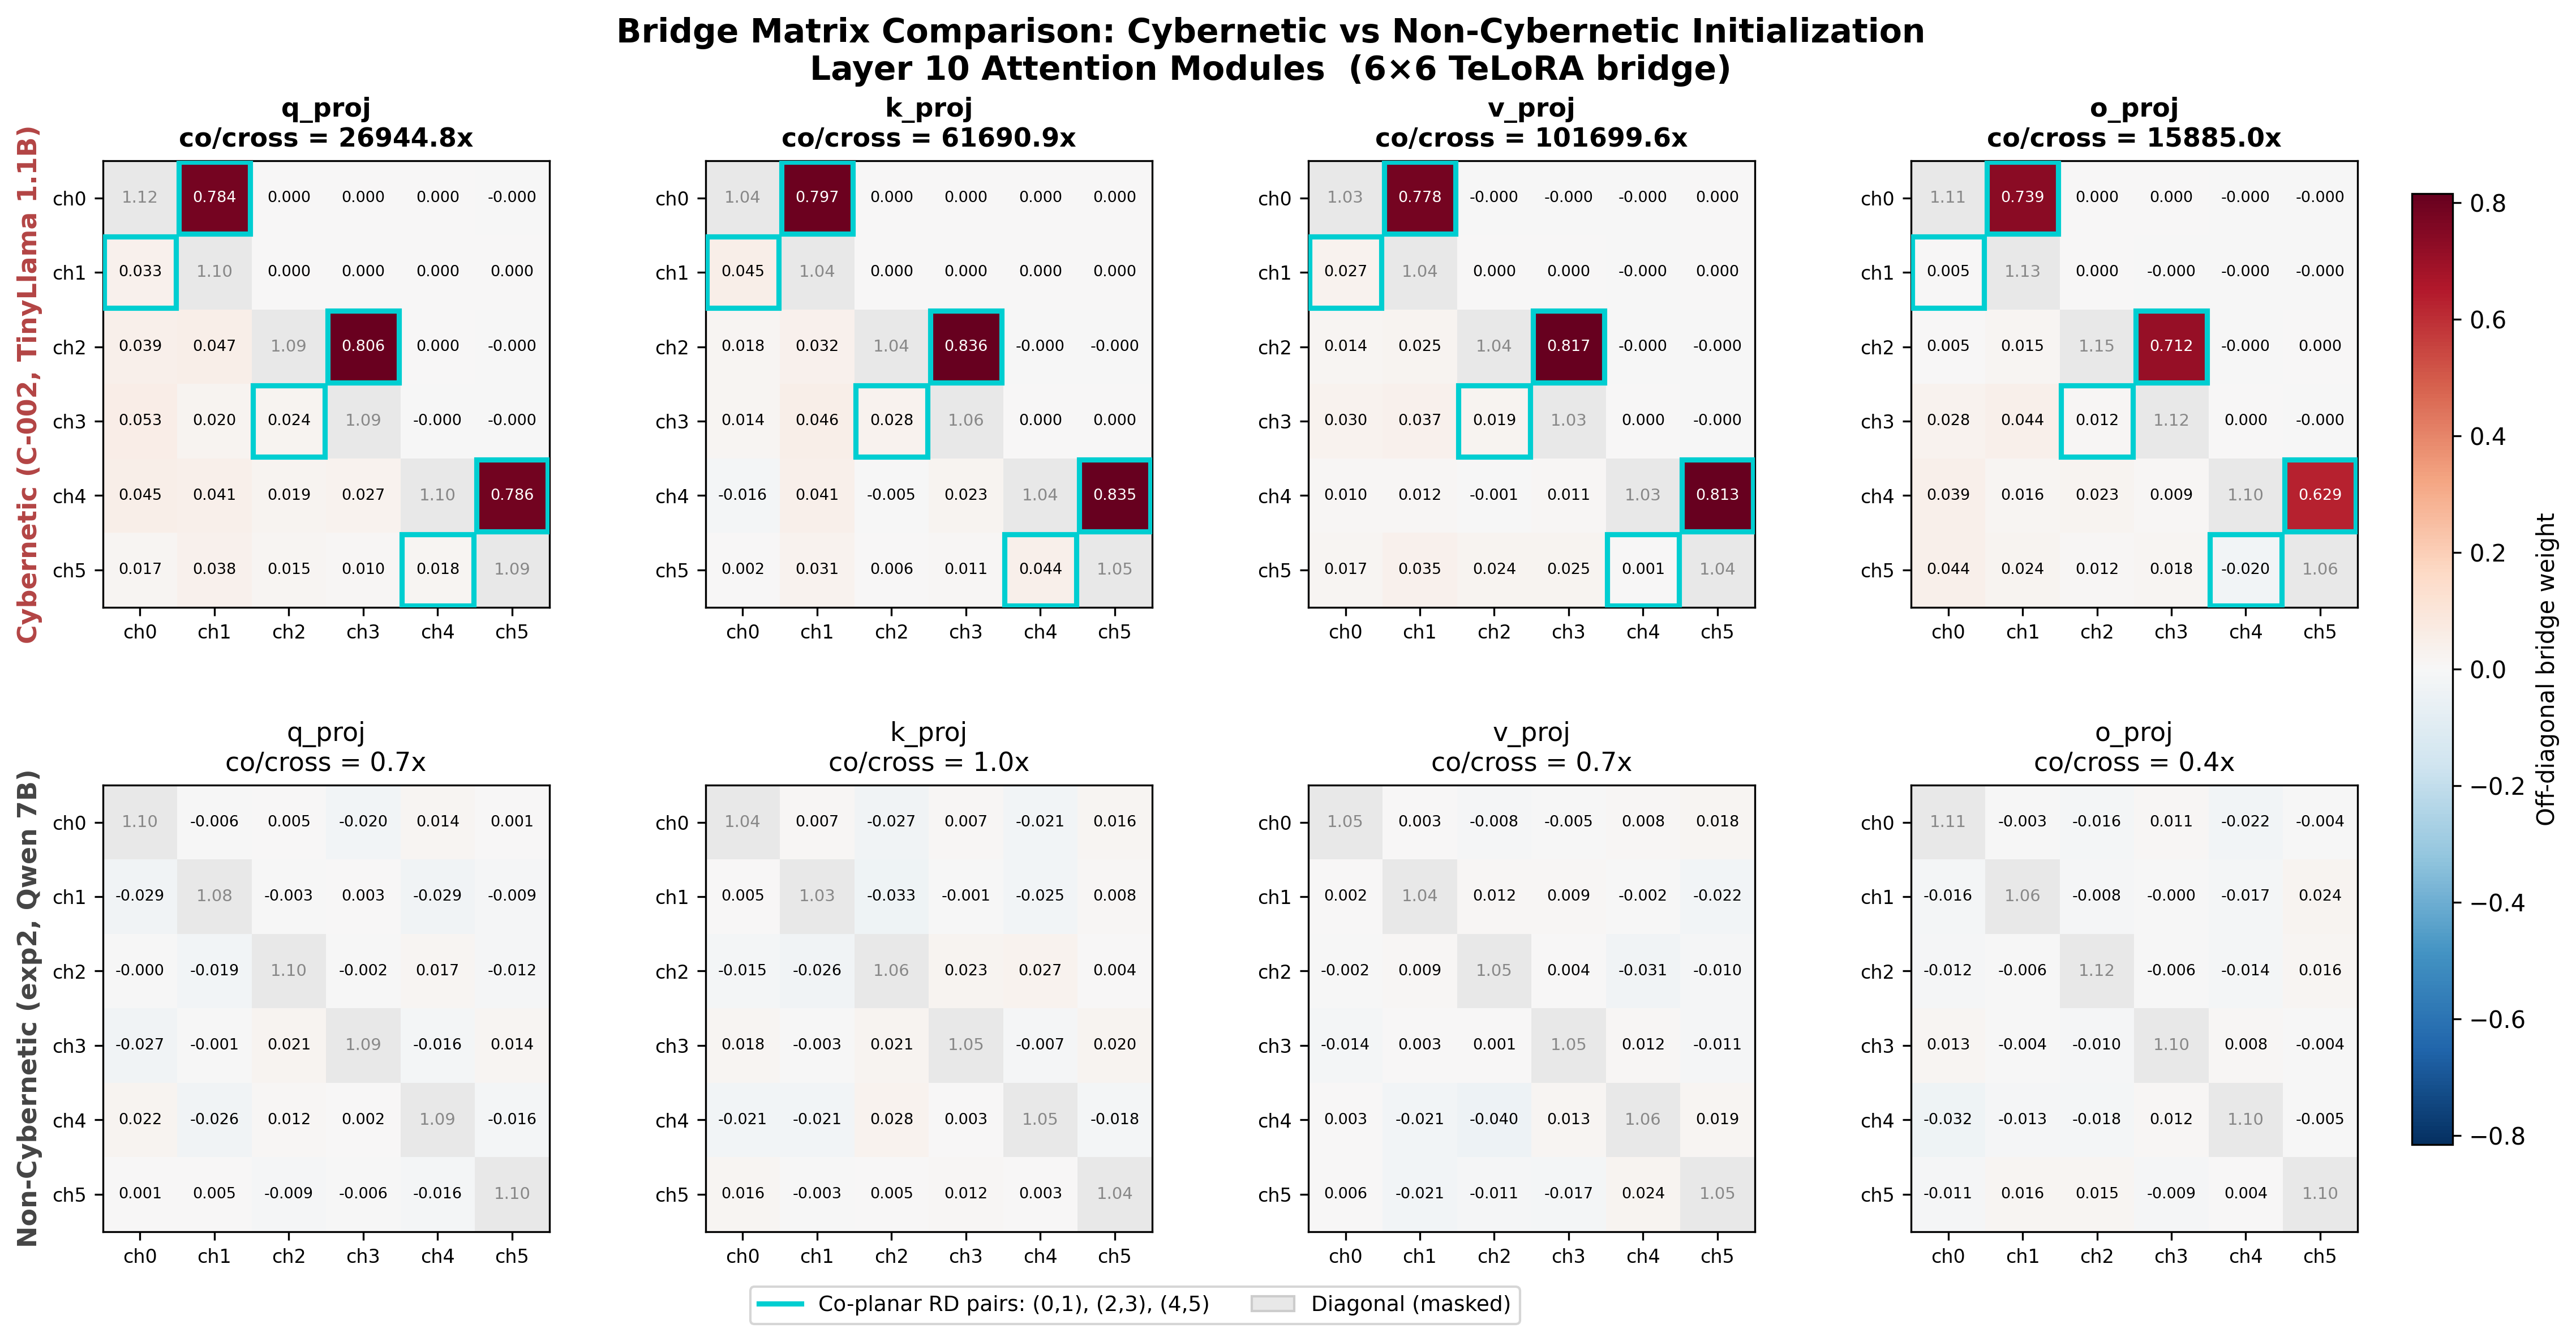
\includegraphics[width=0.85\textwidth]{figures3/fig4-bridge-heatmaps}
\caption{Bridge matrix heatmaps: cybernetic (C-002, left) vs.\
  non-cybernetic (exp2, right) across four module types. Cybernetic
  bridges show clear $3 \times (2 \times 2)$ block-diagonal
  structure; non-cybernetic bridges remain near-identity.}
\label{fig:heatmaps}
\end{figure}


% ===================================================================
\section{Channel Count Ablation}
\label{sec:ablation}

The experiments in Section~\ref{sec:emergence} establish that the
Steersman produces block-diagonal structure at $n = 6$. This section
asks \emph{why} $n = 6$, and what the structure reveals about the
effective dimensionality of the bridge's learned representation.

\subsection{Experimental Design}

We vary the channel count $n \in \{3, 4, 6, 8\}$ while holding the
total LoRA rank fixed at~24. All experiments use TinyLlama~1.1B with
identity initialization and identical hyperparameters
(Section~\ref{sec:setup}). The channel sizes are
$s = 8, 6, 4, 3$ and the bridge parameter counts per module are
$n^2 = 9, 16, 36, 64$.

The critical design element: the contrastive loss component is defined
exclusively for $n = 6$. For $n \neq 6$, the function returns zero.
The spectral loss operates at all channel counts. By comparing $n = 6$
(contrastive + spectral) with $n \in \{3, 4, 8\}$ (spectral only),
we isolate the geometric prior's contribution.

\subsection{Results}

\begin{table}[H]
\centering
\caption{Channel count ablation. Bridge Fiedler = algebraic
  connectivity of the bridge graph. $\rho$ = co-planar/cross-planar
  ratio. Contrastive loss is active only at $n = 6$.}
\label{tab:ablation}
\begin{tabular}{ccrcccc}
\toprule
$n$ & Bridge params/mod & Val Loss & Bridge Fiedler & $\rho$ & BD\% & Contrastive \\
\midrule
3 & 9 & 0.4020 & 0.095 & N/A & N/A & N/A \\
4 & 16 & 0.4022 & 0.092 & ${\sim}1$:1 & 0\% & disabled \\
\textbf{6} & \textbf{36} & \textbf{0.4015} & \textbf{0.00009} & \textbf{70{,}404:1} & \textbf{100\%} & \textbf{active} \\
8 & 64 & 0.4024 & 0.094 & ${\sim}1$:1 & 0\% & disabled \\
\bottomrule
\end{tabular}
\end{table}

\begin{figure}[ht]
\centering
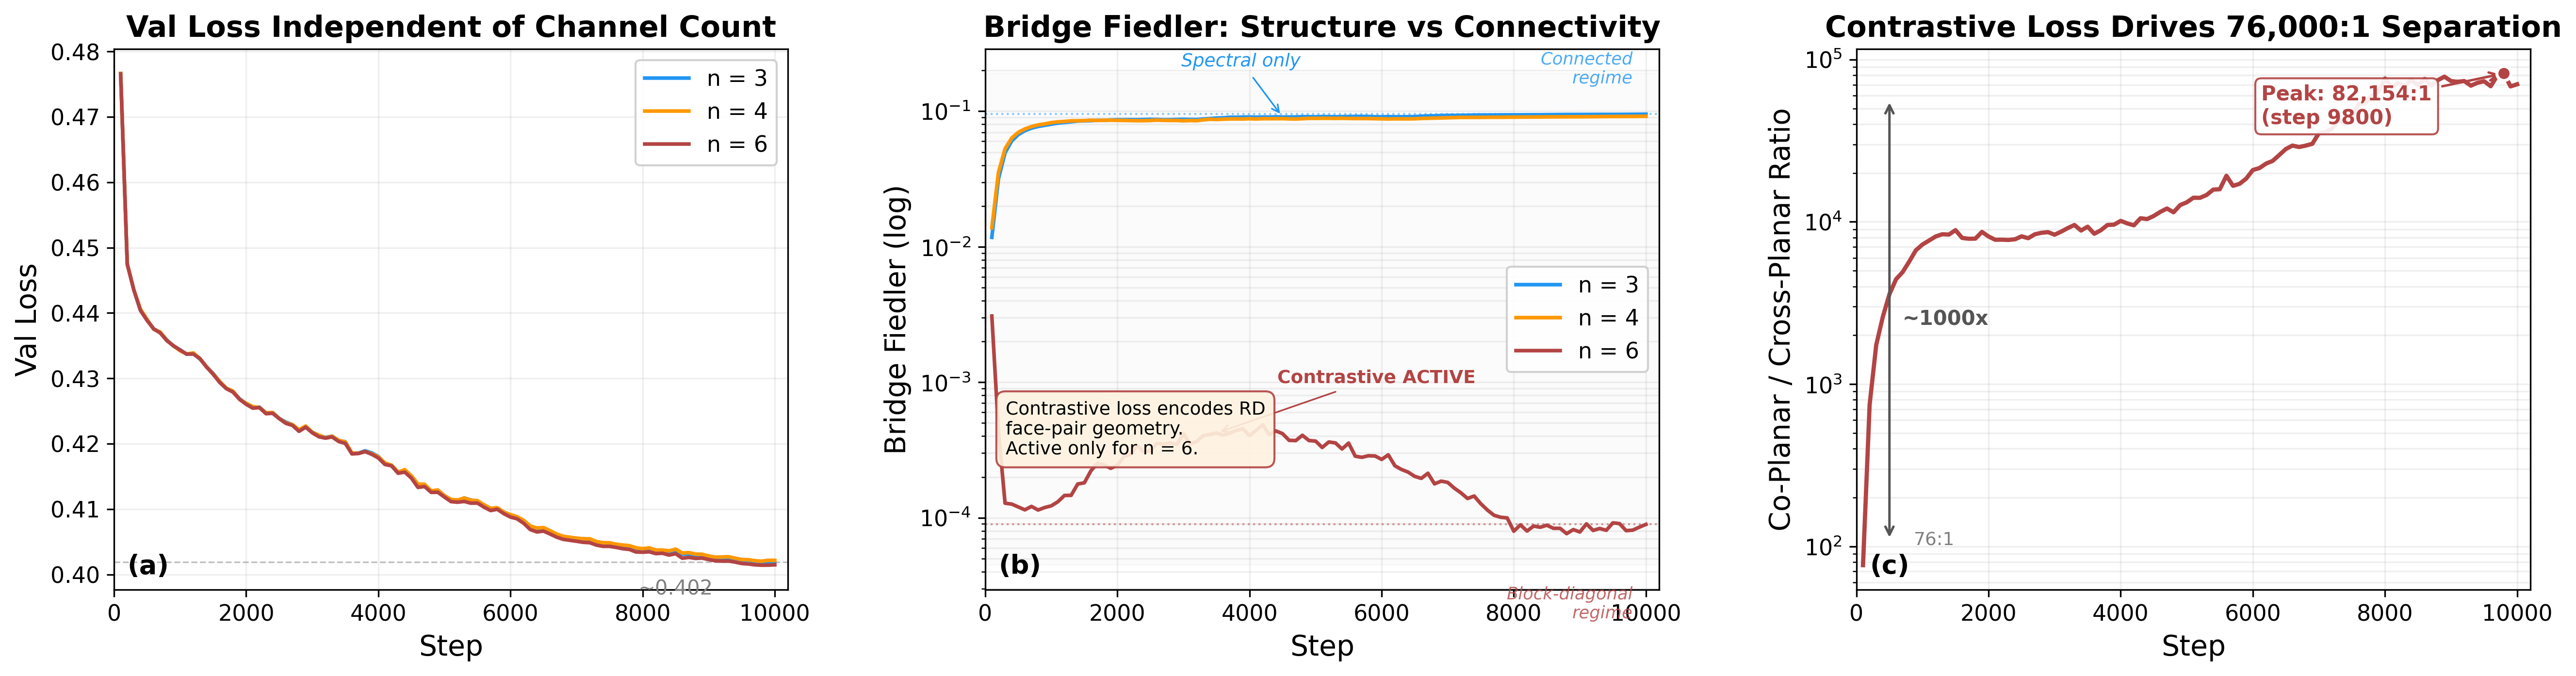
\includegraphics[width=0.85\textwidth]{figures3/fig5-channel-ablation}
\caption{Channel count ablation. Left: validation loss (all channel
  counts within 0.22\%). Center: Bridge Fiedler eigenvalue (log scale;
  $1{,}020\times$ bifurcation between $n = 6$ and all others). Right:
  co-planar/cross-planar ratio ($n = 6$ only; peak 82{,}854:1).}
\label{fig:ablation}
\end{figure}

The results (Figure~\ref{fig:ablation}) separate cleanly along three
dimensions.

\subsubsection{Task Performance Is Insensitive to Channel Count}

Validation loss varies by at most 0.17\% across
$n \in \{3, 4, 6\}$: from 0.4015 ($n = 6$) to 0.4022 ($n = 4$).
Including $n = 8$ (0.4024), the full range is 0.22\%.
Over the full 100-checkpoint trajectory, $n = 3$ and $n = 6$ maintain
a maximum delta of~0.16\%. The task gradient dominates the language
modeling loss surface; bridge topology operates in an orthogonal
subspace.

\subsubsection{Block-Diagonal Structure Emerges Only When the Geometric Prior Is Active}

The Bridge Fiedler eigenvalue bifurcates sharply. At $n = 6$
(contrastive active), Bridge Fiedler converges to~0.00009: the bridge
graph is near-disconnected. At $n \in \{3, 4, 8\}$ (spectral only),
Bridge Fiedler converges to 0.092--0.095: a connected graph with no
preferential topology (Figure~\ref{fig:fiedler}).

The ratio of spectral-only Fiedler (${\sim}0.09$) to
contrastive-active Fiedler ($0.00009$) is approximately
$1{,}020\times$---a bifurcation, not a gradual difference. The
spectral gap at $n = 6$ converges to~0.00006, indicating near-perfect
3-fold eigenvalue degeneracy. At $n = 4$, the spectral gap is~0.559.

\begin{figure}[ht]
\centering
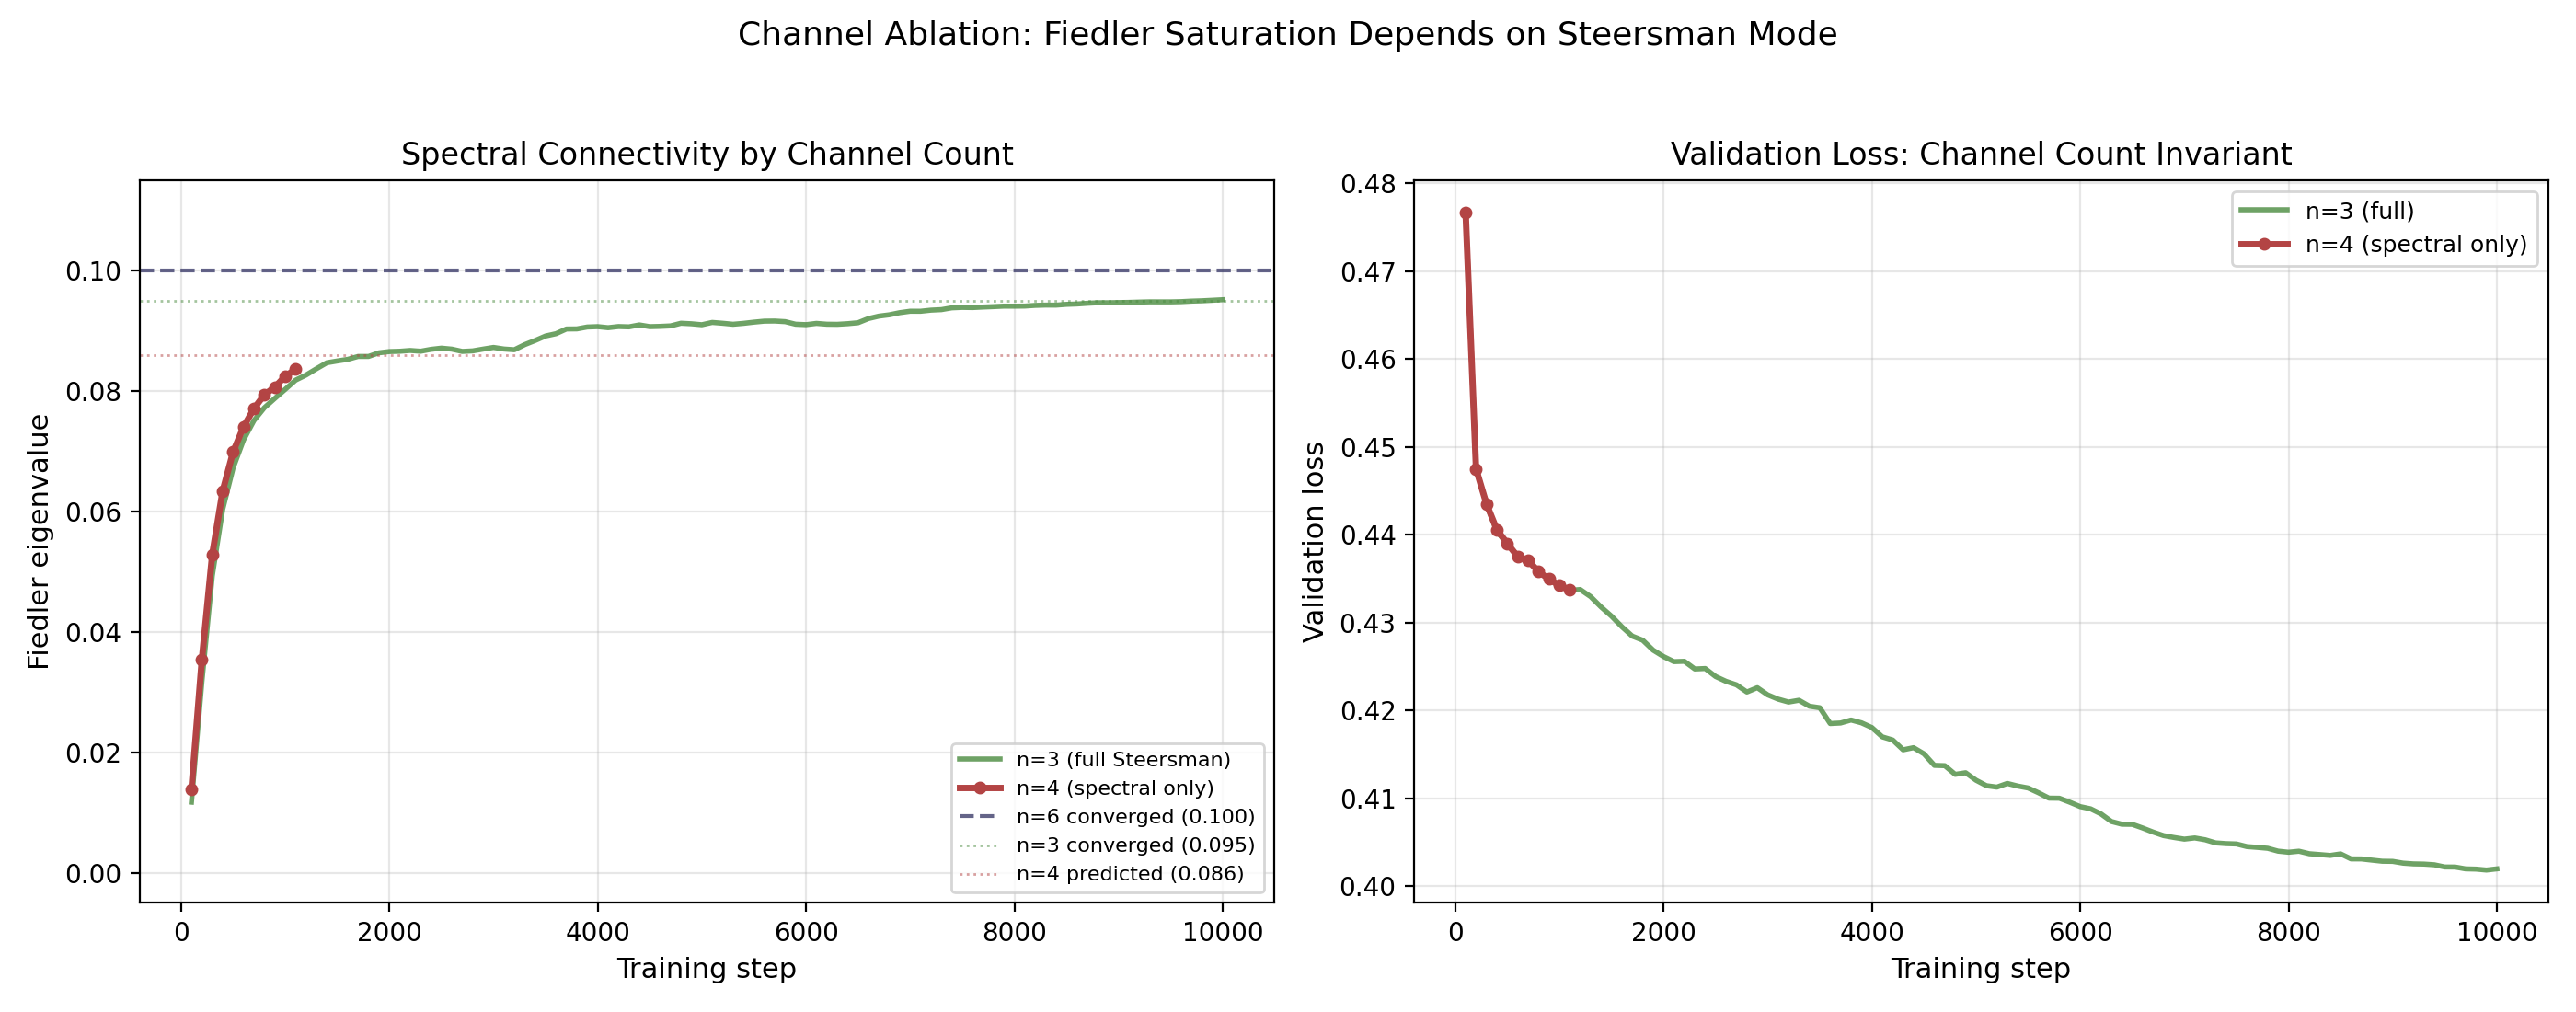
\includegraphics[width=0.75\textwidth]{figures3/fig7-fiedler-saturation}
\caption{Fiedler eigenvalue saturation across channel counts.
  $n = 6$ collapses to~0.00009 under contrastive loss; $n \in \{3,
  4, 8\}$ converge to~$0.092$--$0.095$ under spectral loss alone.
  Also shows validation loss comparison.}
\label{fig:fiedler}
\end{figure}

\subsubsection{The Fiedler Trajectory at $n = 4$: Competing Objectives}

The $n = 4$ experiment reveals non-trivial dynamics. The Bridge
Fiedler trajectory exhibits three phases: (1)~rapid growth
(steps~0--1{,}200, Fiedler rising to~0.084), (2)~a dip
(steps~1{,}200--3{,}000, declining to~0.076---a 9.5\% decrease
despite continued spectral pressure), and (3)~recovery
(steps~3{,}000--10{,}000, climbing to~0.092).

\begin{figure}[ht]
\centering
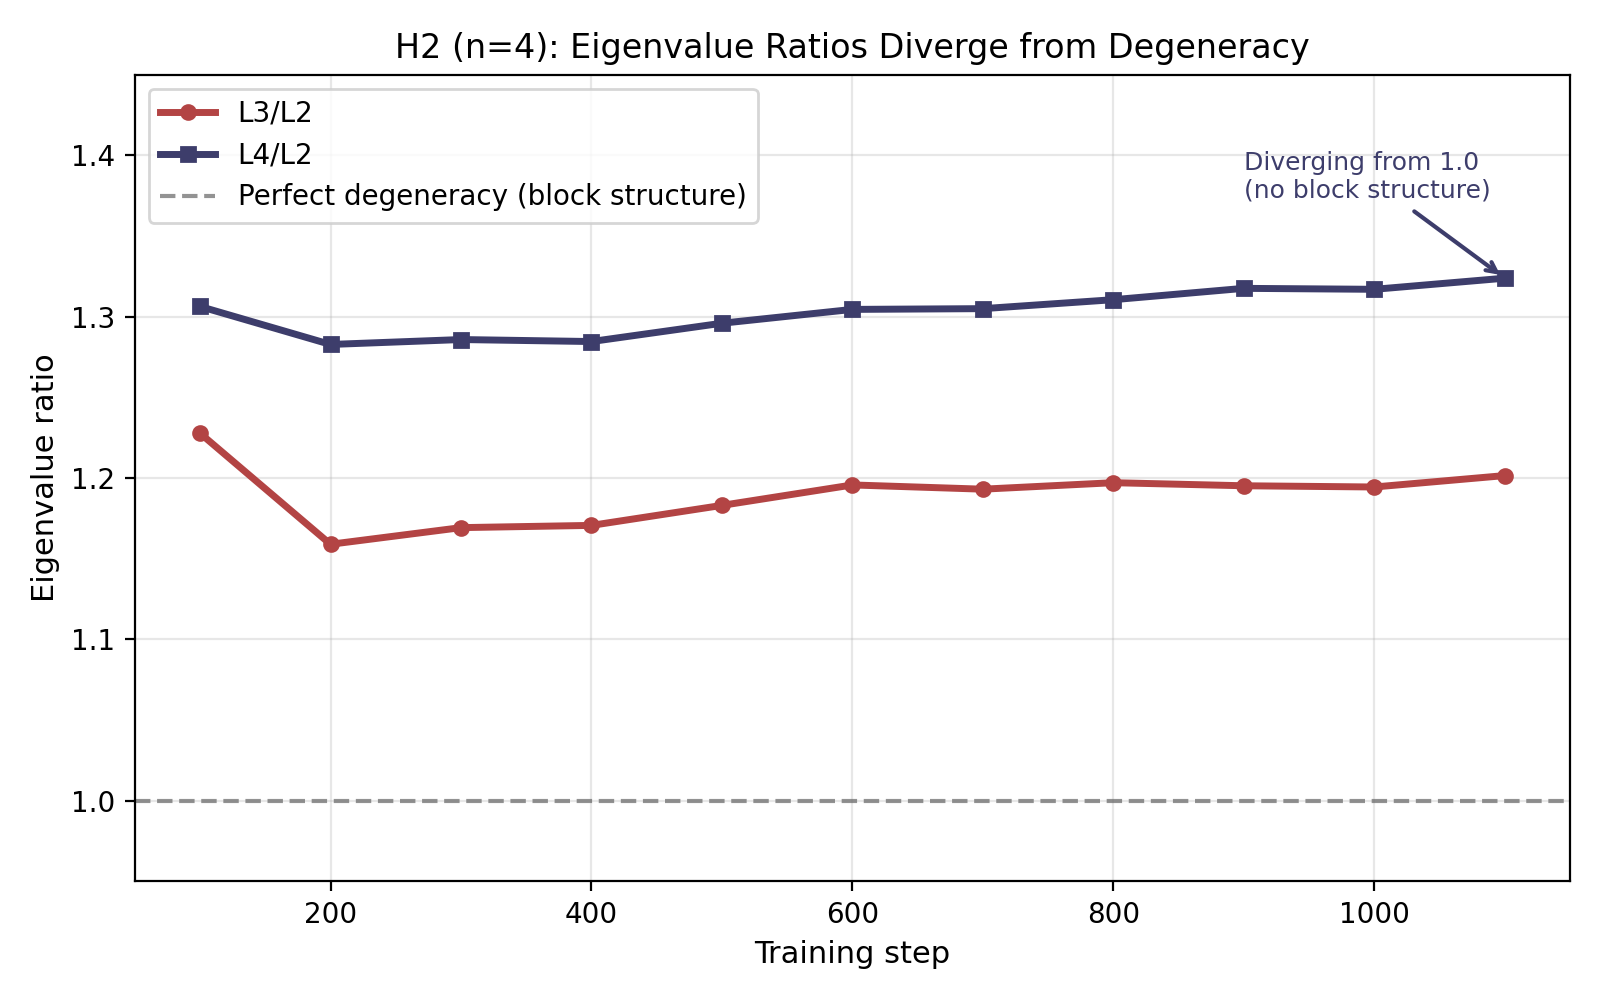
\includegraphics[width=0.65\textwidth]{figures3/fig6-h2-eigenvalues}
\caption{$n = 4$ (H2) eigenvalue ratios diverging from degeneracy.
  The bridge at $n = 4$ develops no block structure---all eigenvalues
  remain distinct.}
\label{fig:h2eigen}
\end{figure}

This three-phase trajectory (Figure~\ref{fig:h2eigen}) is absent at
$n = 6$, where Bridge Fiedler falls monotonically from step~1 onward.
The contrastive loss's gradient toward block structure is strong enough
that the task gradient cannot overcome it.

\subsubsection{Three Regimes of Bridge Behavior}

The ablation reveals three qualitatively distinct regimes:

\textbf{Trivial ($n = 3$).} With only 6~off-diagonal entries,
the bridge has too few degrees of freedom for block structure.
Spectral regularization drives uniform coupling
(Fiedler~0.095).

\textbf{Spectral-only ($n = 4, 8$).} Bridges develop uniform
connectivity (Fiedler~0.092--0.094) with no topological preference.
The spectral loss drives connectivity magnitude but provides no
signal about which entries should grow relative to others.

\textbf{Full Steersman ($n = 6$).} The contrastive loss drives a
$1{,}020\times$ Fiedler bifurcation. Bridge matrices decompose into
three independent $2 \times 2$ blocks. The spectral gap collapses
to~0.00006. The bridge's 15 off-diagonal degrees of freedom reduce
to effectively 3 active dimensions.

\subsection{Effective Rank and Parameter Efficiency}

The Steersman at $n = 6$ discovers a 3-dimensional structure within a
15-dimensional parameter space. The 12~cross-planar entries are driven
to zero; only the 3~co-planar entries carry information. This matches
$n = 3$, which has effectively 3~off-diagonal pairs and achieves
matching task performance.

Concretely: $n = 3$ uses 9~bridge parameters per module (792~total
in TinyLlama), while $n = 6$ uses 36~per module (3{,}168~total)---a
$4\times$ overhead. The additional parameters provide no performance
benefit (validation loss delta ${\leq}\,0.16\%$) but reveal the
internal structure: the system has 3 effective degrees of freedom,
corresponding to the 3~coordinate axes of the rhombic dodecahedron.

The $n = 6$ bridge is a redundant parameterization of a 3-axis
coordinate system. The redundancy is diagnostic: a $3 \times 3$ bridge
achieves the same function but provides no information about which
geometric structure underlies the coupling. The $6 \times 6$ bridge,
by developing block-diagonal structure under the contrastive loss,
reveals that the relevant structure is the 3-axis partition encoded in
the RD geometry.


% ===================================================================
\section{Scale Consistency}
\label{sec:scale}

\subsection{Cross-Scale Comparison}

Block-diagonal structure appears identically at 1.1B (TinyLlama)
and 7B (Qwen2.5). The Qwen~7B experiment (exp3) produces 100\%
block-diagonal bridges with $\rho = 18{,}248$:1. The lower ratio
compared to TinyLlama runs (64{,}000--71{,}000:1) reflects an earlier
code version with less aggressive contrastive weighting, not a
scale-dependent effect.

Per-layer coupling analysis (Figure~\ref{fig:perlayer}) reveals
comparable structure across scales. Both models exhibit the same per-module hierarchy:
$k$\_proj develops the strongest coupling (44{,}000:1 in Qwen~7B;
46{,}570:1 in C-002 TinyLlama), followed by $v$\_proj (44{,}000:1;
24{,}462:1), then $q$\_proj (22{,}477:1; 16{,}708:1), with $o$\_proj
weakest (19{,}080:1; 9{,}116:1). The ordering $k \geq v > q > o$ is
consistent across scales (with $k$ and $v$ tied at Qwen~7B;
Figure~\ref{fig:permodule}), suggesting a shared
architectural pattern.

\begin{figure}[ht]
\centering
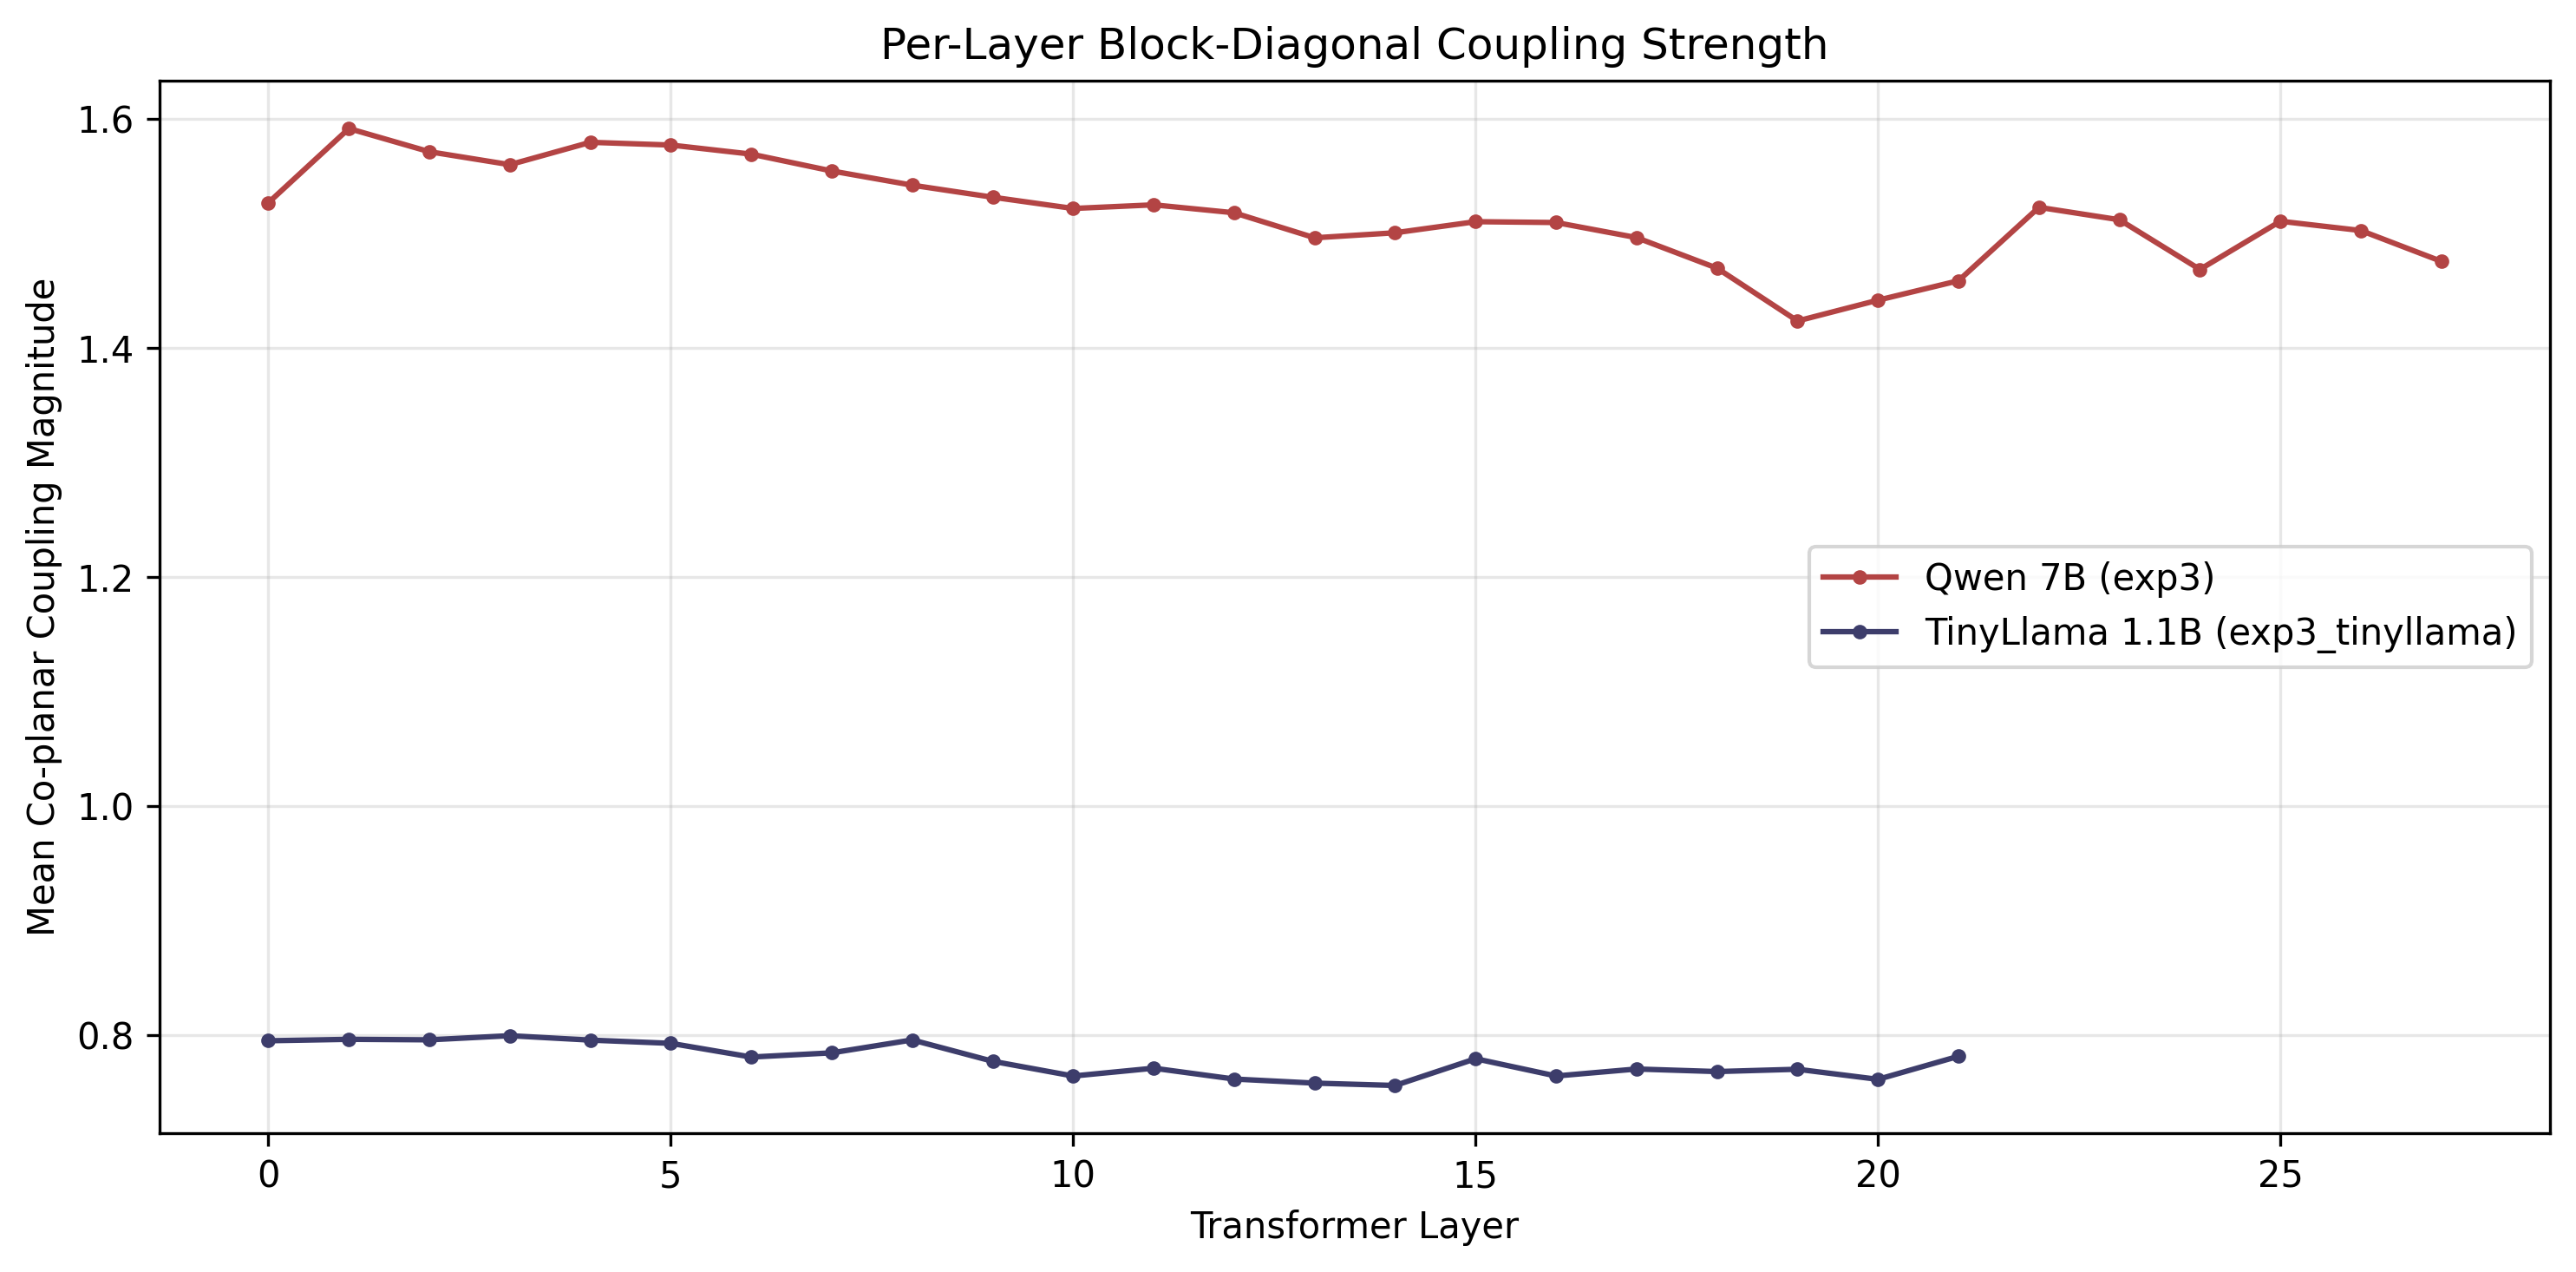
\includegraphics[width=0.75\textwidth]{figures3/fig8-per-layer-coupling}
\caption{Per-layer co-planar coupling: Qwen~7B vs.\ TinyLlama.
  Coupling is uniform across layers to within 5\% in both models, with
  no systematic front-to-back gradient.}
\label{fig:perlayer}
\end{figure}

\begin{figure}[ht]
\centering
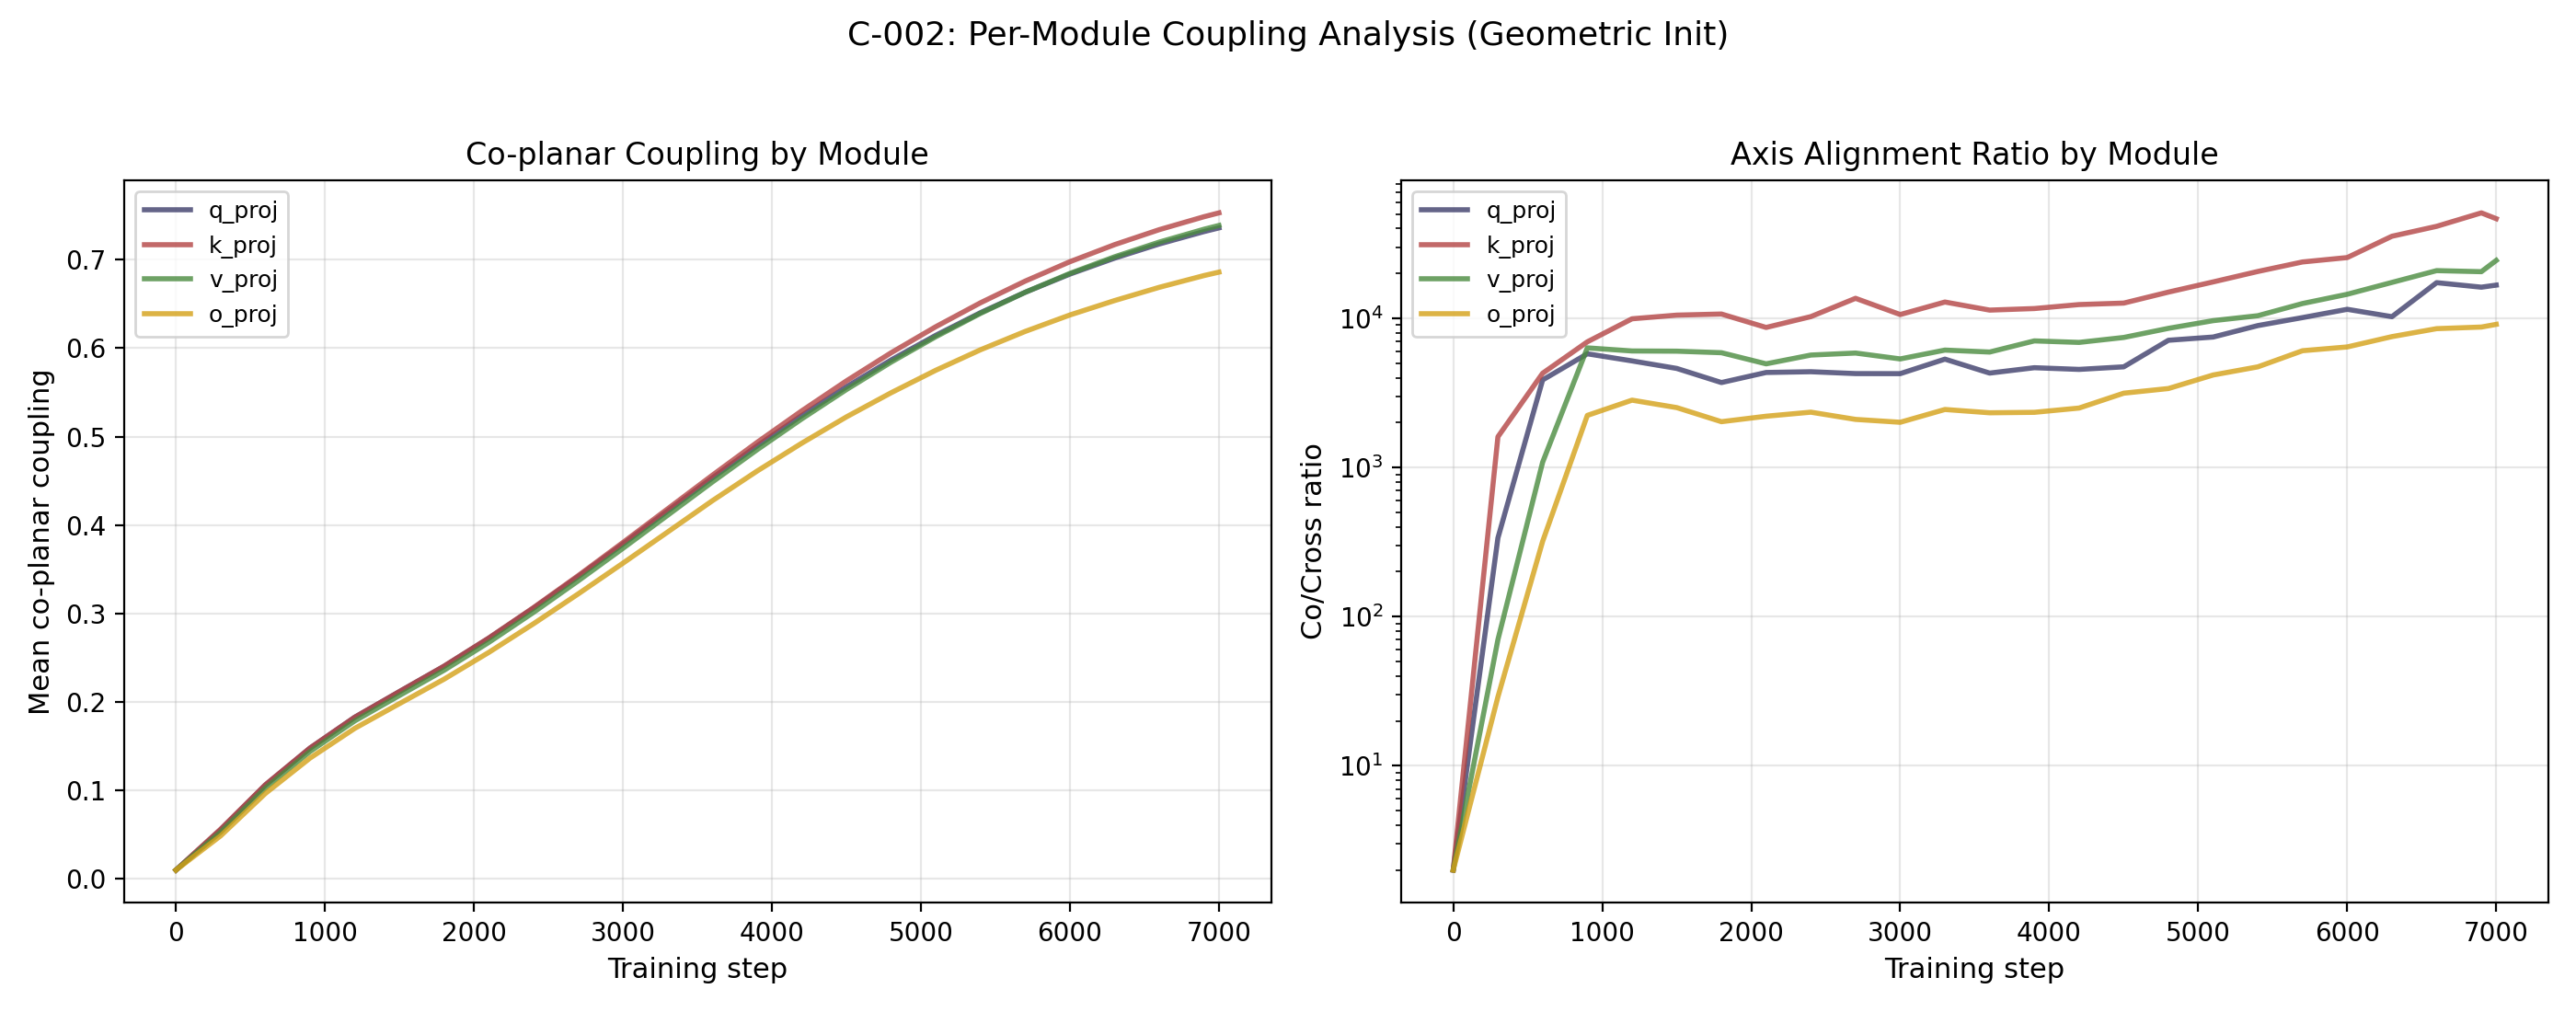
\includegraphics[width=0.65\textwidth]{figures3/fig9-per-module-coupling}
\caption{Per-module coupling hierarchy in C-002 (TinyLlama):
  $k$\_proj $>$ $v$\_proj $>$ $q$\_proj $>$ $o$\_proj. The ordering
  is consistent across scales.}
\label{fig:permodule}
\end{figure}

\subsection{Two Fiedler Metrics}

The analysis employs two distinct applications of the Fiedler
eigenvalue.

\textbf{Bridge Fiedler} measures \emph{within-matrix} connectivity.
For a single bridge matrix~$\mathbf{M}$, the weighted Laplacian
treats $|M_{ij}|$ as edge weights and computes~$\lambda_2$. Low
Bridge Fiedler indicates near-disconnected components. Bridge Fiedler
at $n = 6$ (cybernetic):~0.00009. At $n = 4$ (spectral-only):~0.092.

\textbf{Correlation Fiedler} measures \emph{cross-layer} structural
consistency. For each module type, the flattened bridge matrices
across all layers form $n^2$-dimensional vectors; the pairwise Pearson
correlation matrix's Fiedler eigenvalue measures structural
uniformity across depth.

The Correlation Fiedler converges to~${\sim}0.10$ for cybernetic text
models: 0.102 (Qwen~7B) and 0.101 (TinyLlama). The Holly Battery~14B
(non-cybernetic) has Correlation Fiedler~1.002---near-perfect
cross-layer correlation arising from its near-identity bridges. The
${\sim}0.10$ convergence for cybernetic models indicates that bridge
structure is uniform across layers regardless of model depth or size,
while the Holly value reflects a qualitatively different regime where
minimal bridge perturbations are trivially correlated.

\subsection{The Holly Battery Null Result}

The Holly Battery experiment provides the non-cybernetic control at
14B~scale. Wan~2.1 is fine-tuned with 6-channel RhombiLoRA but
without the Steersman. The adapter achieves 3.8\% lower loss than the
standard LoRA baseline, requires 9.15\,GB less VRAM, and produces
6\% faster inference.

Despite these performance benefits, the Holly Battery bridge matrices
are near-identity: mean off-diagonal magnitude~0.010,
$\rho = 1.07$:1, Bridge Fiedler~${\sim}0.10$. The bridge learns small
perturbations from identity that improve task performance, but these
perturbations are uniformly distributed with no preferential topology.

The Holly result provides additional evidence consistent with the
Steersman as the causal factor, complementing the more controlled
Qwen-family comparison (exp2/exp2.5 without Steersman vs.\ exp3 with
Steersman, where model family, task, and dataset are held constant).


% ===================================================================
\section{Discussion}
\label{sec:discussion}

\subsection{Why Block-Diagonal?}

The contrastive loss provides a strong gradient signal that
differentiates co-planar from cross-planar entries. Once stochastic
perturbations break symmetry, co-planar entries receive positive
reinforcement while cross-planar entries receive negative
reinforcement. The exponential decay of cross-planar coupling
(half-life: 123~steps) reflects self-reinforcing suppression: the
gradient of $-|x|$ has constant magnitude regardless of~$x$,
maintaining pressure until entries reach the computational floor.

The linear growth of co-planar coupling reflects the absence of
saturation in the contrastive reward: there is no target magnitude,
only the directive to maximize~$\rho$. The result is an asymmetric
attractor: entry into the basin (exponential suppression) is fast,
while the attractor's depth (co-planar magnitude) increases
monotonically.

The attractor occupies 3~dimensions of a 15-dimensional parameter
space. The 12~cross-planar directions are exponentially repulsive.
The 3~co-planar directions are linearly attractive. This
asymmetry---3~attractive, 12~repulsive---is a geometric consequence
of the RD face-pair partition.

\subsection{Practical Implications}

\textbf{Diagnostic over-parameterization.} The $n = 6$ bridge uses
$4\times$ more parameters than $n = 3$ but achieves identical task
performance. The excess parameters are diagnostically valuable: they
reveal the 3-axis coordinate structure that $n = 3$ achieves
implicitly. For practitioners: train with $n = 6$ and cybernetic
feedback to discover the bridge's preferred topology, then deploy with
$n = 3$ for parameter efficiency.

\textbf{Cybernetic training as structural discovery.} The Steersman
does not improve task performance (validation loss within 0.17\% of
spectral-only training). Its value is structural: it reveals the
bridge's geometric preferences. The bridge
accepts the RD geometry (100\% BD) while developing no structure
without it (0\% BD without contrastive loss), indicating that the RD
coordinate system is compatible with the adapter's representational
structure under these training conditions.

\textbf{Programmable topology.} The contrastive loss is a topology
selector. The current experiments use RD face-pair geometry. A natural
extension is to test alternative topologies---random partitions,
task-specific pairings, or geometries from other polyhedra---to
determine whether the bridge accepts arbitrary programs or
specifically prefers the RD coordinate structure.

\subsection{Limitations}

\textbf{Single task family.} All experiments use instruction-following
(alpaca-cleaned). The block-diagonal structure may depend on task
type, dataset, or the relationship between task complexity and channel
count.

\textbf{Single bridge architecture.} The bridge is a dense
$n \times n$ matrix. Alternative parameterizations (sparse, symmetric,
orthogonal) may produce different outcomes.

\textbf{Contrastive loss confound.} The contrastive loss is defined
only for $n = 6$. The ablation isolates the contrastive loss as the
mechanism but does not test whether an $n = 4$ or $n = 8$ contrastive
loss (using a different geometric prior) would produce block structure
at those channel counts. The current design confounds channel count
with contrastive availability.

\textbf{No formal null model.} The probability of observing 100\%
block-diagonal structure by chance under the null hypothesis has not
been computed analytically. The empirical null rate is 0\%
(6~non-cybernetic experiments, 570~bridges).

\textbf{Limited scale range.} Three model scales (1.1B, 7B, 14B)
provide evidence, but the 14B result is non-cybernetic only and
differs from the causal LM experiments in model architecture, task,
dataset, and optimizer. Two cybernetic scales are insufficient to
establish a scaling law. A cybernetic experiment at 14B or larger
would confirm that block-diagonal emergence scales to frontier model
sizes.

\textbf{Single seed.} All experiments use random seed~42. While
the binary block-diagonal classification (100\% vs.\ 0\%) is robust
given the magnitude of the effect, specific numerical
quantities---coupling ratios, half-life estimates, per-module
hierarchies---are single-seed observations and may vary under
different initializations of the LoRA parameters and data ordering.

\textbf{Ablation scale.} The channel-count ablation (Section~\ref{sec:ablation}) was conducted at 1.1B
only. Whether the $n = 6$ bifurcation replicates at 7B or larger
is untested.

\textbf{Steersman sensitivity.} The Steersman's control parameters
(Table~\ref{tab:steersman}) are hand-tuned. No sensitivity analysis
has been conducted; the robustness of block-diagonal emergence to
variations in feedback thresholds, gain constants, and weight bounds
is untested.

\subsection{Connection to Broader Literature}

Block-diagonal structure in neural network weight matrices has been
observed in modular networks~\cite{clune2013}, lottery
tickets~\cite{frankle2019lottery}, and sparse
MoE~\cite{fedus2022switch}. In all prior cases, the block structure
arises from architectural constraints or regularization penalties. The
present work demonstrates block-diagonal emergence through a purely
cybernetic mechanism: second-order feedback that monitors spectral
properties without constraining the bridge matrix itself.

The Steersman's design draws on cybernetic control
theory~\cite{ashby1956, wiener1948}: a sense-decide-actuate loop that
maintains homeostasis. The three control laws operate independently,
each monitoring a different aspect of the bridge's evolving state.
This architecture is simpler than learned
meta-optimizers~\cite{andrychowicz2016} or neural architecture
search~\cite{zoph2017neural}---fixed control laws with adaptive
thresholds---yet sufficient to drive a strong structural attractor.

The effective dimensionality finding---3~active dimensions from 15
available---connects to the literature on intrinsic dimensionality of
optimization landscapes~\cite{li2018visualizing, aghajanyan2021}.
Those works estimate intrinsic dimensionality of the full weight
update; here, we observe it directly in the bridge's learned
structure. The effective rank~(3) equaling the number of
coordinate axes suggests that the Steersman aligns dimensionality
with a specific geometric basis.


% ===================================================================
\section{Conclusion}
\label{sec:conclusion}

The learnable bridge in multi-channel LoRA, under cybernetic feedback,
discovers the 3-axis coordinate geometry of the rhombic dodecahedron.
This geometry is not imposed---it emerges as a robust attractor of a
feedback loop that encodes face-pair relationships through a
contrastive loss and monitors spectral connectivity through a reactive
controller.

The finding holds across every experimental axis tested.
Six cybernetic experiments at $n = 6$ produce 100\% block-diagonal
structure across 42{,}500+ bridges; non-cybernetic controls
produce~0\%. Three initialization strategies---including one that
actively opposes the target topology---converge to the same attractor
within 200~steps. Validation loss is insensitive to bridge topology
(0.17\% maximum delta across $n \in \{3, 4, 6\}$). The contrastive
loss, encoding RD face-pair geometry, is both necessary and
sufficient at $n = 6$: removing it (at $n \in \{3, 4, 8\}$) produces
$1{,}020\times$ higher Bridge Fiedler with 0\% block structure.

The effective dimensionality of the discovered structure is
effectively~3---the number of coordinate axes, not the number of faces.
The 6-channel bridge is a redundant parameterization that reveals
structure; the 3-channel bridge achieves the same function without
revealing it.

These results suggest that multi-channel LoRA adapters are receptive to
geometric structure when it is encoded in the training objective.
Cybernetic feedback---even a simple reactive controller with fixed
control laws---is sufficient to discover and stabilize these
preferences. The Steersman provides no task performance benefit; its
contribution is structural transparency. The bridge, under feedback,
tells us what it has learned.

\paragraph{Availability.}
Source code:
\url{https://github.com/promptcrafted/rhombic}.\\
Package: \url{https://pypi.org/project/rhombic/} (v0.3.0, 312~tests).\\
Reproduction: install \texttt{rhombic} and run the training scripts
with \texttt{seed=42}.


% ===================================================================
\appendix
\section{Experimental Details}
\label{app:details}

\subsection{Common Hyperparameters}

\begin{table}[H]
\centering
\caption{Common hyperparameters across all experiments.}
\label{tab:hyperparams}
\begin{tabular}{lr}
\toprule
Parameter & Value \\
\midrule
Optimizer & AdamW \\
Weight decay & 0.01 \\
Base learning rate & $2 \times 10^{-4}$ \\
LR schedule & Cosine decay after linear warmup \\
Warmup steps & 200 \\
Batch size & 2 \\
Gradient accumulation & 8 \\
Effective batch size & 16 \\
Max gradient norm & 1.0 \\
LoRA rank ($r$) & 24 \\
LoRA $\alpha$ & 16 \\
LoRA dropout & 0.0 \\
Target modules & $W_Q, W_K, W_V, W_O$ \\
Dataset & alpaca-cleaned (90/10 train/val split) \\
Max sequence length & 512 \\
Precision & bfloat16 \\
Gradient checkpointing & Enabled \\
Random seed & 42 \\
Steersman feedback interval & 100 steps \\
\bottomrule
\end{tabular}
\end{table}

\subsection{Steersman Hyperparameters}

\begin{table}[H]
\centering
\caption{Steersman control parameters.}
\label{tab:steersman}
\begin{tabular}{lr}
\toprule
Parameter & Value \\
\midrule
Initial contrastive weight ($w_c$) & 0.1 \\
Max contrastive weight ($w_c^{\max}$) & 0.5 \\
Initial spectral weight ($w_s$) & 0.05 \\
Max spectral weight ($w_s^{\max}$) & 0.2 \\
Target Fiedler ($\lambda_2^*$, initial) & 0.1 \\
Fiedler decline threshold & $-0.001$ \\
Stagnation threshold & 0.02 \\
Deviation growth threshold & 0.05 \\
Min bridge LR multiplier & 0.1 \\
Sliding window size & 5 measurements \\
Spectral boost gain & $10.0 \times |\text{trend}|$ \\
Contrastive increment & 0.02 per intervention \\
Stability dampen floor & 0.8 \\
Spectral decay target & $0.5 \times w_s^{\text{base}}$ \\
Fiedler target tracking rate & 0.1 \\
\bottomrule
\end{tabular}
\end{table}

\subsection{Per-Experiment Configuration}

\begin{table}[H]
\centering
\caption{Per-experiment details.}
\label{tab:perexp}
\small
\begin{tabular}{llclcrr}
\toprule
ID & Model & $n$ & Init & Steps & Machine & Wall Time \\
\midrule
exp3 & Qwen2.5-7B-Instruct & 6 & identity & 12{,}900 & RTX 6000 Ada 48\,GB & ${\sim}36$h \\
exp3\_tiny & TinyLlama-1.1B-Chat & 6 & identity & 10{,}000 & RTX 6000 Ada & ${\sim}12$h \\
C-001 & TinyLlama-1.1B-Chat & 6 & identity & 4{,}000 & RTX 6000 Ada & ${\sim}5$h \\
C-002 & TinyLlama-1.1B-Chat & 6 & geometric & 10{,}000 & RTX 6000 Ada & ${\sim}12$h \\
C-003 & TinyLlama-1.1B-Chat & 6 & corpus & 10{,}000 & RTX 6000 Ada & ${\sim}12$h \\
H1 & TinyLlama-1.1B-Chat & 3 & identity & 10{,}000 & RTX 4090 16\,GB & ${\sim}10$h \\
H2 & TinyLlama-1.1B-Chat & 4 & identity & 10{,}000 & RTX 4090 & ${\sim}10$h \\
H3 & TinyLlama-1.1B-Chat & 6 & identity & 10{,}000 & RTX 4090 & ${\sim}10$h \\
H4 & TinyLlama-1.1B-Chat & 8 & identity & 10{,}000 & RTX 4090 & ${\sim}10$h \\
Holly & Wan-2.1-14B & 6 & identity & 10 epochs & A100 80\,GB & ${\sim}12$h \\
\bottomrule
\end{tabular}
\end{table}

\noindent\textbf{Holly Battery configuration note.} The Holly Battery
uses Prodigy optimizer (d0 = $10^{-4}$, weight decay 0.01) instead of
AdamW; fine-tunes a video diffusion model on proprietary video data
(not alpaca-cleaned); targets attention layers in the Wan~2.1
transformer blocks; and trains for 10~epochs (${\sim}600$ steps at
batch size 1, gradient accumulation 4). No Steersman is applied. The
Holly Battery serves as a non-cybernetic control at 14B scale and is
not intended to be independently reproduced; the more controlled
comparison is within the Qwen family (exp2/exp2.5 without Steersman
vs.\ exp3 with Steersman), where model family, task, and dataset are
held constant.

\subsection{Bridge Parameter Counts}

\begin{table}[H]
\centering
\caption{Bridge parameter counts for TinyLlama-1.1B (88 modules).}
\label{tab:bridgeparams}
\begin{tabular}{cccrr}
\toprule
$n$ & Channel size ($s = r/n$) & Params/module ($n^2$) & Total bridge params & \% of LoRA params \\
\midrule
3 & 8 & 9 & 792 & 0.01\% \\
4 & 6 & 16 & 1{,}408 & 0.02\% \\
6 & 4 & 36 & 3{,}168 & 0.04\% \\
8 & 3 & 64 & 5{,}632 & 0.07\% \\
\bottomrule
\end{tabular}
\end{table}

\subsection{Hardware}

\begin{table}[H]
\centering
\caption{Hardware.}
\label{tab:hardware}
\begin{tabular}{llrl}
\toprule
Machine & GPU & VRAM & Role \\
\midrule
Local workstation & NVIDIA RTX 6000 Ada & 48\,GB & C-001/2/3, exp3, exp3\_tiny \\
Hermes server & NVIDIA RTX 4090 & 16\,GB & H1--H4 (channel ablation) \\
RunPod cloud & NVIDIA A100 & 80\,GB & Holly Battery (14B) \\
\bottomrule
\end{tabular}
\end{table}

\subsection{Block-Diagonal Detection Criteria}

A bridge matrix $\mathbf{M}$ is classified as block-diagonal if both:
(1)~$\rho > 10$ (co-planar/cross-planar ratio exceeds~10:1), and
(2)~$\max_{(i,j) \in \mathcal{X}} |M_{ij}| < 10^{-3}$ (all
cross-planar entries below threshold). These thresholds are
conservative: typical cybernetic bridges at convergence have
$\rho > 60{,}000$:1 and cross-planar maximum $< 10^{-5}$.


% ===================================================================
\section*{Acknowledgments}

The author thanks Araminta K for partnership in Promptcrafted.
Portions of the codebase and manuscript were developed with AI
assistance (Claude, Anthropic).

% ===================================================================
\bibliographystyle{plainnat}
\bibliography{rhombic-paper3}

\end{document}
